% Standalone wrapper for compiling the chapter on its own.
% In the full book, copy the package list into the book preamble and % Chapter 9: biological networks.
% Requires: amsmath, amssymb, bm, graphicx, booktabs, subcaption,
% tikz (arrows.meta, positioning, calc, decorations.pathreplacing, fit, shapes.geometric), natbib.
% Computed figures and figures/network_stats.tex are produced by scripts/make_figures.py;
% figures/slides/ holds figures taken from the lecture slides.

\providecommand{\R}{\mathbb{R}}
\providecommand{\E}{\mathbb{E}}
\providecommand{\Normal}{\mathcal{N}}
\providecommand{\argmax}{\operatorname*{arg\,max}}
\providecommand{\argmin}{\operatorname*{arg\,min}}
\providecommand{\vy}{\mathbf{y}}
\providecommand{\vx}{\mathbf{x}}
\providecommand{\mX}{\mathbf{X}}
\providecommand{\mI}{\mathbf{I}}
\providecommand{\vb}{\boldsymbol{\beta}}
\providecommand{\veps}{\boldsymbol{\epsilon}}
\providecommand{\vp}{\mathbf{p}}
\providecommand{\vg}{\mathbf{g}}
\providecommand{\ind}{\mathbf{1}}
\providecommand{\mA}{\mathbf{A}}
\providecommand{\mTheta}{\boldsymbol{\Theta}}
\providecommand{\mSigma}{\boldsymbol{\Sigma}}
\providecommand{\hSigma}{\hat{\boldsymbol{\Sigma}}}
\providecommand{\mGamma}{\boldsymbol{\Gamma}}
\providecommand{\veta}{\boldsymbol{\eta}}
\providecommand{\vc}{\mathbf{c}}
\providecommand{\vz}{\mathbf{z}}
\providecommand{\vpi}{\boldsymbol{\pi}}
\providecommand{\tr}{\operatorname{tr}}
\providecommand{\cor}{\operatorname{cor}}
\providecommand{\Cov}{\operatorname{Cov}}
\providecommand{\Var}{\operatorname{Var}}
\providecommand{\Bern}{\operatorname{Bernoulli}}
\providecommand{\Cat}{\operatorname{Categorical}}
\providecommand{\Dir}{\operatorname{Dirichlet}}
\providecommand{\indep}{\perp\!\!\!\perp}

% generated by scripts/make_figures.py
\providecommand{\corrFiveSeven}{0.36}
\providecommand{\pcorFiveSeven}{0.06}
\providecommand{\glassoEdges}{12}
\providecommand{\pathRank}{29}
\providecommand{\pathBestLambda}{0.36}
\providecommand{\pathBestEdges}{41}
\providecommand{\pathBestTrue}{18}
\providecommand{\btwNodes}{150}
\providecommand{\btwEdges}{687}
\providecommand{\btwDensity}{0.061}
\providecommand{\btwDiameter}{12}
\providecommand{\btwClustering}{0.64}
\providecommand{\btwMaxBC}{0.19}
\providecommand{\maxDegER}{18}
\providecommand{\maxDegBA}{163}
\providecommand{\sbmARI}{1.00}
\providecommand{\sbmEtaHat}{0.03 & 0.03 & 0.30 & 0.02 \\ 0.03 & 0.39 & 0.04 & 0.03 \\ 0.30 & 0.04 & 0.02 & 0.03 \\ 0.02 & 0.03 & 0.03 & 0.37}


\providecommand{\chaptertoc}{}
\chapter{Biological networks}
\label{ch:networks}
\chaptertoc

``Tell me with whom you consort and I will tell you who you are,'' wrote Goethe in his \textit{Maxims and Reflections}. Much of network biology rests on the same idea, often called \emph{guilt by association}: the function of a gene, protein or metabolite can be inferred from the other entities it is connected to. A network, or graph, is a set of nodes and a set of edges between pairs of nodes. In biology the word ``network'' is used for many different things, and the nodes and edges mean different things in each case. On meeting a network in a paper, the first question to ask is what kind of network it is: what are the nodes, what does an edge mean, is it directed, and how was it measured or inferred?

This chapter has three parts. The first surveys the main kinds of biological network: gene regulatory, protein-protein interaction, genetic interaction, metabolic and signaling networks. The second shows how to estimate an undirected network from gene expression data using partial correlations and the graphical lasso, and how to share information when estimating networks for many related tissues. The third treats a network as data in its own right: summary properties from graph theory, and probabilistic models of network structure, the stochastic blockmodel and its mixed membership extension.

%======================================================================
\section{Kinds of biological network}
\label{sec:network_types}
%======================================================================

\subsection{Gene regulatory networks}

Earlier chapters described how transcription factors (TFs) bind DNA near a gene's promoter and increase or decrease its transcription. TFs are proteins, encoded by genes, so their own expression must also be regulated. A TF may activate a set of target genes, some of which are themselves TFs that activate further targets, and some targets feed back to regulate the TF that started the cascade (Figure~\ref{fig:grn_schematic}). Negative feedback of this kind prevents runaway overexpression. The result is a \emph{gene regulatory network} (GRN), in which nodes are genes and a directed edge $A\to B$ means that the product of gene $A$ regulates the expression of gene $B$. Edges are signed: by convention an ordinary arrow denotes activation (up-regulation) and a bar-headed arrow denotes repression (down-regulation).

\begin{figure}[tbp]
  \centering
  \begin{tikzpicture}[>=Stealth, every node/.style={font=\small},
      gene/.style={draw, rounded corners, minimum width=1.6cm, minimum height=0.6cm, fill=blue!8}]
    \node[gene, fill=orange!25] (tf) at (0,0) {TF};
    \node[gene] (a) at (3.2,1.1) {gene A};
    \node[gene] (b) at (3.2,0) {gene B};
    \node[gene, fill=orange!25] (c) at (3.2,-1.1) {gene C (TF)};
    \node[gene] (d) at (6.6,-0.5) {gene D};
    \node[gene] (e) at (6.6,-1.7) {gene E};
    \draw[->, thick] (tf) -- (a);
    \draw[->, thick] (tf) -- (b);
    \draw[->, thick] (tf) -- (c);
    \draw[->, thick] (c) -- (d);
    \draw[-{Bar[width=6pt]}, thick] (c) -- (e);
    \draw[-{Bar[width=6pt]}, thick, red!70!black] (c.south) to[out=-100, in=-90, looseness=1.3] node[below, pos=0.5] {negative feedback} (tf.south);
  \end{tikzpicture}
  \caption{A gene regulatory network. A transcription factor (TF) activates genes A, B and C. Gene C encodes another TF, which activates D, represses E, and represses the first TF, closing a negative feedback loop. Ordinary arrows denote activation, bar-headed arrows repression.}
  \label{fig:grn_schematic}
\end{figure}

The classical way to map a GRN is one gene at a time: knock down or knock out a gene and measure how the expression of other genes changes. Pooled CRISPR screens with single-cell RNA-seq readout, such as Perturb-seq~\citep{dixit2016} and CROP-seq~\citep{datlinger2017}, scale this up. A pool of cells is transduced with a library of guide RNAs so that each cell carries, typically, one perturbation that knocks down (or activates) one gene. The guide identity is recorded in each cell's sequencing library, and single-cell RNA-seq then measures the downstream effect on the whole transcriptome. Figure~\ref{fig:dixit} shows a regulatory network among immune TFs inferred from such a screen in dendritic cells. Early screens perturbed tens to hundreds of genes; genome-scale Perturb-seq has since perturbed every expressed gene in a cell line~\citep{replogle2022}.

\begin{figure}[tbp]
  \centering
  \includegraphics[width=0.5\linewidth]{slides/dixit_perturbseq_network.png}
  \caption{A regulatory network among transcription factors in mouse dendritic cells stimulated with lipopolysaccharide, inferred from a Perturb-seq screen. Blue arrows denote activation and red bar-headed arrows repression; grey regions mark modules M1--M4 of co-functional regulators. Reproduced from \citet{dixit2016}.}
  \label{fig:dixit}
\end{figure}

The readout in these experiments is almost always RNA. Protein levels can be measured for far fewer genes, and some regulation acts on translation or on splicing (Section~\ref{sec:te_ir}), so RNA is not an ideal readout, but it is the one we can measure most completely. Inferring a causal GRN remains hard even with perturbation data. Of the roughly 20{,}000 human protein-coding genes perhaps 8{,}000 are expressed in a given cell type, so the GRN is in principle an $8000\times 8000$ matrix of regulatory effects.

An older strategy reduces the number of parameters in two steps. Genes are first grouped into \emph{modules}, clusters of co-expressed genes, by clustering or by a matrix factorization such as non-negative matrix factorization (Chapter 8) that lets modules share genes. A network is then inferred between modules, or from regulators to modules, rather than between individual genes. Module networks~\citep{segal2003} learned regulators of yeast modules with probabilistic graphical models from observational expression data. \citet{mostafavi2018} applied a similar approach to RNA-seq from the aging human brain, inferring a network of a few tens of modules and linking some of them to amyloid and tau pathology and to cognitive decline. Bayesian network learning of this kind has become less common as perturbation data have grown.

\subsection{Protein-protein interaction networks}

To many biologists ``network'' means a \emph{protein-protein interaction} (PPI) network. The nodes are proteins and an undirected edge means that the two proteins physically bind. Proteins often act in complexes: RNA polymerase II, for example, transcribes DNA to RNA together with a large set of general transcription factors and the Mediator complex, all physically associated with it. Experimental methods usually start from one protein and find its partners, so interaction maps are assembled from many labor-intensive experiments. The results are collected in databases, of which the largest are BioGRID~\citep{stark2006} and STRING~\citep{szklarczyk2019}. STRING also includes predicted functional associations, for example from co-expression and text mining, not only physical binding.

PPI networks are best thought of as having a high false negative rate and a modest false positive rate. An edge in a curated database usually reflects a real interaction, but many true interactions are missing because nobody has tested them, and well-studied proteins have more recorded partners than less-studied ones. Figure~\ref{fig:scz} shows an example network built around genes associated with schizophrenia, which combined known interactions with several hundred newly predicted ones~\citep{ganapathiraju2016}.

\begin{figure}[tbp]
  \centering
  \includegraphics[width=0.65\linewidth]{slides/schizophrenia_interactome.png}
  \caption{A protein-protein interaction network centered on genes associated with schizophrenia (labelled nodes). Known interactions are combined with interactions predicted computationally. Reproduced from \citet{ganapathiraju2016}.}
  \label{fig:scz}
\end{figure}

\paragraph{Yeast two-hybrid screens.} The yeast two-hybrid (Y2H) assay~\citep{fields1989} tests whether two proteins X and Y bind. It uses the yeast transcription factor Gal4, which has two separable parts: a DNA binding domain (BD) that recognizes an upstream activating sequence (UAS), and an activation domain (AD) that recruits the transcriptional machinery. Neither part alone activates transcription. The ``bait'' protein X is fused to the BD and the ``prey'' protein Y to the AD, each expressed from its own plasmid. If X and Y interact, they bring the BD and AD together at the UAS and a reporter gene is transcribed, for example one needed for growth on a selective medium (Figure~\ref{fig:y2h}). Screening a bait against a library of prey reveals its binding partners.

\begin{figure}[tbp]
  \centering
  \begin{tikzpicture}[>=Stealth, every node/.style={font=\small}]
    % plasmids
    \draw[thick] (0,3.0) circle (0.55);
    \draw[line width=3pt, black] (0,3.0) ++(60:0.55) arc (60:110:0.55);
    \draw[line width=3pt, gray] (0,3.0) ++(115:0.55) arc (115:200:0.55);
    \node at (0.45,3.75) {X}; \node at (-0.95,2.95) {BD};
    \node at (0,2.15) {bait plasmid};
    \draw[thick] (4,3.0) circle (0.55);
    \draw[line width=3pt, black] (4,3.0) ++(60:0.55) arc (60:110:0.55);
    \draw[line width=3pt, gray] (4,3.0) ++(115:0.55) arc (115:200:0.55);
    \node at (4.45,3.75) {Y}; \node at (3.05,2.95) {AD};
    \node at (4,2.15) {prey plasmid};
    % fusion proteins
    \node[draw, fill=gray!50, minimum width=0.9cm, minimum height=0.45cm] (bd1) at (-0.3,1.1) {BD};
    \node[draw, ellipse, minimum width=0.7cm, minimum height=0.9cm] (x1) at (0.5,1.3) {X};
    \node[draw, ellipse, minimum width=0.7cm, minimum height=0.9cm] (y1) at (3.65,1.2) {Y};
    \node[draw, circle, fill=gray!50, minimum size=0.75cm] (ad1) at (4.4,0.95) {AD};
    \draw[->] (0,1.95) -- (0,1.75);
    \draw[->] (4,1.95) -- (4,1.75);
    % complex on DNA
    \draw[thick] (-1.2,-1) -- (7.5,-1);
    \node[draw, fill=white, minimum width=1.3cm, minimum height=0.45cm] (uas) at (-0.3,-1) {UAS};
    \node[draw, fill=white, minimum width=2.3cm, minimum height=0.45cm] (rep) at (5.6,-1) {reporter gene};
    \node[draw, fill=gray!50, minimum width=0.9cm, minimum height=0.45cm] (bd2) at (-0.3,-0.48) {BD};
    \node[draw, ellipse, minimum width=0.7cm, minimum height=0.9cm] (x2) at (0.55,-0.25) {X};
    \node[draw, ellipse, minimum width=0.7cm, minimum height=0.9cm] (y2) at (1.25,-0.25) {Y};
    \node[draw, circle, fill=gray!50, minimum size=0.75cm] (ad2) at (2.0,-0.55) {AD};
    \draw[->, thick] (4.45,-0.75) -- (4.45,-0.2) -- (6.6,-0.2) node[above, pos=0.5] {transcription};
    \draw[->, thick] (2.0,0.7) -- (2.0,0.1) node[midway, right] {if X binds Y};
  \end{tikzpicture}
  \caption{The yeast two-hybrid assay. The bait protein X is fused to the Gal4 DNA binding domain (BD) and the prey Y to the Gal4 activation domain (AD). If X and Y bind, the BD and AD are brought together at the upstream activating sequence (UAS) and the reporter gene is transcribed. After a slide figure of the assay~\citep{fields1989}.}
  \label{fig:y2h}
\end{figure}

\subsection{Genetic interaction networks}

Budding yeast, \textit{Saccharomyces cerevisiae}, is single-celled but, like us, a eukaryote, with a nucleus and much of the same core cellular machinery. A surprising amount of biology is conserved between yeast and humans; some of the proteins whose misfolding damages neurons in neurodegenerative disease are also toxic to yeast, for example. Yeast grows fast and is easy to manipulate genetically, which makes possible experiments that would be impractical in mammalian cells.

One such experiment maps \emph{genetic interactions}. A collection of yeast strains each lacking one of the roughly 6{,}000 genes (or carrying a weakened allele of an essential gene) can be crossed systematically to make double mutants, and the fitness of each double mutant measured from the size of its colony on an agar plate. \citet{costanzo2016} constructed and measured roughly 23 million double mutants. The colony size $C_{ij}$ of the double mutant lacking genes $i$ and $j$ is modelled as
\begin{equation}
  C_{ij} = f_{ij}\times t\times s_{ij}\times e,
\end{equation}
where $f_{ij}$ is the double-mutant fitness, $t$ is the growth time, $s_{ij}$ collects systematic experimental effects (such as position on the plate) and $e$ is noise. After estimating and removing $t$ and $s_{ij}$, the double-mutant fitness is compared with the product of the single-mutant fitnesses $f_i$ and $f_j$,
\begin{equation}
  f_{ij} = f_if_j + \epsilon_{ij}.
\end{equation}
The multiplicative model $f_if_j$ is the expected fitness if the two genes act independently, so that each deletion reduces growth by a fixed factor. The deviation $\epsilon_{ij}$ is the \emph{genetic interaction score}. A negative score, with the extreme case of synthetic lethality, means the double mutant is sicker than expected; this often happens when the two genes act in parallel pathways that can compensate for each other. A positive score means the double mutant is healthier than expected, as when both genes act in the same pathway or complex, so that losing one already disables it.

The matrix of scores $\epsilon_{ij}$ defines a weighted network over genes. More informative still is the \emph{profile} of each gene, its row of interaction scores with all other genes. Genes with similar profiles tend to have similar functions. Connecting genes whose profiles are correlated and laying out the resulting network gives the functional map of the yeast cell in Figure~\ref{fig:costanzo}, in which clusters correspond to cellular processes.

\begin{figure}[tbp]
  \centering
  \includegraphics[width=0.75\linewidth]{slides/costanzo_functional_map.png}
  \caption{A global map of the yeast cell from genetic interaction profiles. Each dot is a gene; genes with similar genetic interaction profiles are placed near each other, and colored clusters are labelled by the biological process enriched in them. Reproduced from \citet{costanzo2016}.}
  \label{fig:costanzo}
\end{figure}

\subsection{Metabolic networks}

Metabolism is the set of chemical reactions by which a cell converts nutrients into energy and building blocks. A metabolic network has metabolites as nodes and reactions, catalyzed by enzymes, as edges; more precisely it is a bipartite graph between metabolites and reactions, or a hypergraph, since a reaction can take several substrates to several products. Pathways such as glycolysis, the citric acid cycle and fatty acid synthesis are paths through this network (Figure~\ref{fig:metabolic}). Curated metabolic pathways for many organisms are available in KEGG~\citep{kanehisa2000}.

\begin{figure}[tbp]
  \centering
  \includegraphics[width=0.8\linewidth]{slides/metabolic_metro_map.png}
  \caption{The core metabolic network drawn as a metro map. Stations are metabolites and lines are pathways. Image by Bert Chan, Hong Kong (``Metabolic Metro Map'', Wikimedia Commons).}
  \label{fig:metabolic}
\end{figure}

\subsection{Signaling networks}

Signaling networks transmit information from outside the cell to the nucleus. A ligand, such as a growth factor, binds a receptor on the cell surface, which triggers a cascade of protein modifications inside the cell, eventually changing the activity of TFs and hence gene expression (Figure~\ref{fig:signaling}). The most common modification is \emph{phosphorylation}: an enzyme called a \emph{kinase} transfers a phosphate group from ATP to a target protein, changing its shape and switching it on or off, and a \emph{phosphatase} removes the phosphate again. A cascade such as Ras$\to$Raf$\to$MEK$\to$ERK is a chain of kinases, each phosphorylating and activating the next. Signaling networks are central to cancer biology. Many oncogenes, such as \textit{RAS} and \textit{BRAF}, encode members of growth signaling pathways whose mutations make the pathway constitutively active, and many targeted cancer drugs are kinase inhibitors.

\begin{figure}[tbp]
  \centering
  \includegraphics[width=0.85\linewidth]{slides/signaling_pathways.png}
  \caption{Major signaling pathways of a mammalian cell. Receptors at the cell membrane (orange) receive external signals such as growth factors, cytokines and death factors; cascades of protein interactions and phosphorylation in the cytoplasm relay the signal to gene regulation in the nucleus (pink), controlling proliferation and apoptosis. Source: Wikimedia Commons, signal transduction pathways diagram (source and license to be confirmed).}
  \label{fig:signaling}
\end{figure}

\subsection{Co-expression networks}

The networks above are measured, or curated from many experiments. A \emph{co-expression network} is instead inferred from expression data: nodes are genes, and an undirected edge means that the expression levels of the two genes are associated across samples. Genes regulated by the same factors will be correlated, so a co-expression network can be read as a network of co-regulation. The simplest construction connects pairs of genes whose correlation exceeds a threshold. The trouble is that correlation does not distinguish direct from indirect association. If gene $C$ regulates both $A$ and $B$, then $A$ and $B$ are correlated even though neither affects the other. The rest of the first half of this chapter develops a better approach based on partial correlation.

%======================================================================
\section{Networks of expression and splicing}
\label{sec:te_ir}
%======================================================================

Gene expression is not the only quantity a regulatory network can act on. Most human genes produce several \emph{isoforms}, transcripts that differ in which exons they include, through alternative splicing (Chapter 10). Splicing is controlled by \emph{splicing factors}, RNA-binding proteins that promote or repress the use of particular exons. \citet{saha2017} built co-expression networks from GTEx RNA-seq data~\citep{gtex2015} whose nodes are of two types. For each gene, the \emph{total expression} (TE) is the summed expression of all its isoforms. For each isoform, the \emph{isoform ratio} (IR) is its expression divided by the TE of its gene, so the IRs of a gene are non-negative and sum to one.

Table~\ref{tab:te_ir} shows why both are needed. A splicing regulator changes how a gene's transcripts are spliced. When it is abundant, most transcripts of a target gene are isoform 1; when it is scarce, more are isoform 2. The total expression of the target does not change, so a network built on TE alone cannot see this regulation, while the isoform ratios capture it.

\begin{table}[tbp]
  \centering
  \caption{Total expression (TE) and isoform ratios (IR) of a target gene with two isoforms, at high and low levels of a splicing regulator. Counts are numbers of transcripts. The regulator changes the isoform ratios but not the total expression. After an example in \citet{saha2017}.}
  \label{tab:te_ir}
  \begin{tabular}{lccccc}
    \toprule
    Splicing regulator & Isoform 1 & Isoform 2 & TE & IR$_1$ & IR$_2$ \\
    \midrule
    high & 4 & 1 & 5 & 0.8 & 0.2 \\
    low  & 2 & 3 & 5 & 0.4 & 0.6 \\
    \bottomrule
  \end{tabular}
\end{table}

The data for one tissue form a matrix $\mX\in\R^{N\times P}$, with $N$ samples (individuals) as rows and $P$ features as columns, the TE features of all genes followed by the IR features of all isoforms. The goal is a sparse undirected network over the $P$ features. The pipeline (Figure~\ref{fig:twn_pipeline}) computes the $P\times P$ sample covariance matrix, estimates a sparse inverse covariance, or precision, matrix from it with the graphical lasso, and reads the network off the non-zero entries of the precision matrix. The next two sections explain why the precision matrix is the right object and how the graphical lasso estimates it.

\begin{figure}[tbp]
  \centering
  \begin{tikzpicture}[>=Stealth, every node/.style={font=\small}]
    % data matrix
    \fill[blue!15] (0,0) rectangle (1.05,2.1);
    \fill[yellow!35] (1.05,0) rectangle (2.1,2.1);
    \draw (0,0) grid[step=0.35] (2.1,2.1);
    \node[above] at (0.525,2.1) {\footnotesize TE};
    \node[above] at (1.575,2.1) {\footnotesize IR};
    \node[left, rotate=90, anchor=south] at (-0.15,1.05) {samples ($N$)};
    \node[below] at (1.05,-0.05) {data $\mX$};
    \draw[->, thick] (2.4,1.05) -- (3.1,1.05);
    % covariance
    \begin{scope}[xshift=3.4cm]
      \fill[gray!20] (0,0) rectangle (2.1,2.1);
      \draw (0,0) grid[step=0.35] (2.1,2.1);
      \node[below, align=center] at (1.05,-0.05) {sample covariance\\$\hSigma$, $P\times P$};
    \end{scope}
    \draw[->, thick] (5.8,1.05) -- node[above, align=center] {\footnotesize graphical\\[-2pt]\footnotesize lasso} (7.1,1.05);
    % sparse precision
    \begin{scope}[xshift=7.4cm]
      \foreach \i/\j in {0/0,1/1,2/2,3/3,4/4,5/5,0/3,3/0,1/4,4/1,1/2,2/1,4/5,5/4}
        \fill[gray!45] (0.35*\i,2.1-0.35*\j-0.35) rectangle (0.35*\i+0.35,2.1-0.35*\j);
      \draw (0,0) grid[step=0.35] (2.1,2.1);
      \node[below, align=center] at (1.05,-0.05) {sparse precision\\$\hat\mTheta$, $P\times P$};
    \end{scope}
    \draw[->, thick] (9.8,1.05) -- (10.4,1.05);
    % network
    \begin{scope}[xshift=11.1cm, yshift=0.2cm, every node/.style={font=\footnotesize, inner sep=1.5pt}]
      \node[draw, circle, fill=blue!15] (t1) at (0,1.6) {1};
      \node[draw, circle, fill=blue!15] (t2) at (1.2,1.6) {2};
      \node[draw, circle, fill=blue!15] (t3) at (1.6,0.6) {3};
      \node[draw, rectangle, fill=yellow!35] (i4) at (0,0.3) {4};
      \node[draw, rectangle, fill=yellow!35] (i5) at (0.8,-0.2) {5};
      \node[draw, rectangle, fill=yellow!35] (i6) at (1.9,-0.4) {6};
      \draw (t1) -- (i4); \draw (t2) -- (i5); \draw (t2) -- (t3); \draw (i5) -- (i6);
      \node[below, font=\small] at (0.9,-0.6) {network};
    \end{scope}
  \end{tikzpicture}
  \caption{Inferring a network of total expression (TE, circles) and isoform ratio (IR, squares) features. The $N\times P$ data matrix gives a $P\times P$ sample covariance matrix; the graphical lasso estimates a sparse precision matrix whose non-zero off-diagonal entries (grey) are the edges of the network. After \citet{saha2017}.}
  \label{fig:twn_pipeline}
\end{figure}

%======================================================================
\section{Partial correlation}
\label{sec:partial_corr}
%======================================================================

\subsection{Direct and indirect association}

Consider five genes $A,B,C,D,E$. Suppose $C$ is a transcription factor that regulates both $A$ and $B$. Then $A$ and $B$ will be correlated across samples even if there is no direct relationship between them. We want an edge between $A$ and $B$ only if they remain associated after accounting for everything else that is measured. The \emph{partial correlation} of $A$ and $B$ given $C,D,E$ formalizes this. Let $x_{nA}$ be the expression of gene $A$ in sample $n$, and regress $x_A$ on the other genes,
\begin{equation}
  x_{nA} = \sum_{g\in\{C,D,E\}}\beta_gx_{ng} + \epsilon_{nA}, \qquad n=1,\dots,N.
\end{equation}
Fitting by ordinary least squares (Chapter 1) gives $\hat\vb$ and residuals $\hat\epsilon_{nA}=x_{nA}-\sum_g\hat\beta_gx_{ng}$, the part of $x_A$ that $C,D,E$ cannot explain. Doing the same for $B$ gives residuals $\hat\epsilon_{nB}$. The sample partial correlation is the correlation of the residuals,
\begin{equation}
  \cor(A,B\mid C,D,E) = \cor\left(\hat\epsilon_A,\hat\epsilon_B\right).
\end{equation}
If $C$ alone explains the association between $A$ and $B$, the residuals are uncorrelated and the partial correlation is near zero.

Running two regressions for each of the $P(P-1)/2$ pairs of genes would be expensive. It turns out that all partial correlations can be read off a single matrix, the inverse of the covariance matrix.

\subsection{Partial correlations from the precision matrix}

Let $\vx\in\R^P$ be a random vector, one sample of the expression of $P$ genes, with $\vx\sim\Normal(\mathbf{0},\mSigma)$. The data are centered so the mean is zero. $\mSigma\in\R^{P\times P}$ is the covariance matrix and $\mTheta=\mSigma^{-1}\in\R^{P\times P}$ is the \emph{precision matrix}, with entries $\theta_{ij}$. Split the coordinates into a block $1=\{A,B\}$ of size 2 and a block $2$ of the remaining $P-2$ genes, and partition
\begin{equation}
  \vx = \begin{pmatrix}\vx_1\\ \vx_2\end{pmatrix},\qquad
  \mSigma = \begin{pmatrix}\mSigma_{11} & \mSigma_{12}\\ \mSigma_{21} & \mSigma_{22}\end{pmatrix},\qquad
  \mTheta = \begin{pmatrix}\mTheta_{11} & \mTheta_{12}\\ \mTheta_{21} & \mTheta_{22}\end{pmatrix},
\end{equation}
where $\mSigma_{11},\mTheta_{11}$ are $2\times 2$, $\mSigma_{12},\mTheta_{12}$ are $2\times(P-2)$ and $\mSigma_{22},\mTheta_{22}$ are $(P-2)\times(P-2)$.

The population version of regressing $\vx_1$ on $\vx_2$ uses the coefficients that minimize expected squared error, $\mathbf{B}=\mSigma_{12}\mSigma_{22}^{-1}$, a $2\times(P-2)$ matrix. (This is the population analogue of $(\mX^\top\mX)^{-1}\mX^\top\vy$: setting the derivative of $\E\|\vx_1-\mathbf{B}\vx_2\|^2$ to zero gives $\mathbf{B}\mSigma_{22}=\mSigma_{12}$.) The residual $\veps_1=\vx_1-\mathbf{B}\vx_2$ has covariance
\begin{align}
  \Cov(\veps_1) &= \mSigma_{11} - \mathbf{B}\mSigma_{21} - \mSigma_{12}\mathbf{B}^\top + \mathbf{B}\mSigma_{22}\mathbf{B}^\top \nonumber\\
  &= \mSigma_{11} - \mSigma_{12}\mSigma_{22}^{-1}\mSigma_{21},
\end{align}
the \emph{Schur complement} of $\mSigma_{22}$ in $\mSigma$. For Gaussian $\vx$ this is also the covariance of the conditional distribution of $\vx_1$ given $\vx_2$, which is $\Normal(\mathbf{B}\vx_2,\,\mSigma_{11}-\mSigma_{12}\mSigma_{22}^{-1}\mSigma_{21})$.

The block matrix inversion formula states that the top-left block of the inverse of a partitioned matrix is the inverse of this Schur complement,
\begin{equation}
  \mTheta_{11} = \left(\mSigma_{11}-\mSigma_{12}\mSigma_{22}^{-1}\mSigma_{21}\right)^{-1}.
\end{equation}
(To check, multiply $\mSigma$ by $\mTheta$ and use $\mTheta_{21}=-\mSigma_{22}^{-1}\mSigma_{21}\mTheta_{11}$, which follows from the bottom-left block of $\mSigma\mTheta=\mI$.) So $\Cov(\veps_1)=\mTheta_{11}^{-1}$. Writing out the inverse of the $2\times2$ block,
\begin{equation}
  \mTheta_{11}^{-1} = \begin{pmatrix}\theta_{AA} & \theta_{AB}\\ \theta_{AB} & \theta_{BB}\end{pmatrix}^{-1}
  = \frac{1}{\theta_{AA}\theta_{BB}-\theta_{AB}^2}\begin{pmatrix}\theta_{BB} & -\theta_{AB}\\ -\theta_{AB} & \theta_{AA}\end{pmatrix}.
\end{equation}
The correlation of the two residuals is the off-diagonal entry divided by the square root of the product of the diagonal entries; the determinant cancels and
\begin{equation}
  \rho_{AB\mid\text{rest}} = \cor(\epsilon_A,\epsilon_B) = -\frac{\theta_{AB}}{\sqrt{\theta_{AA}\theta_{BB}}}.
  \label{eq:partial_corr}
\end{equation}
The partial correlation of every pair of variables, given all the others, is the corresponding entry of the precision matrix, rescaled by the diagonal and with its sign flipped. In particular, $\rho_{AB\mid\text{rest}}=0$ exactly when $\theta_{AB}=0$.

The same block formula with block $1=\{A\}$ alone relates the precision matrix to the regression of one gene on all the others. Using $\mTheta_{21}=-\mSigma_{22}^{-1}\mSigma_{21}\mTheta_{11}$ with $\mTheta_{11}=\theta_{AA}$ a scalar, the regression coefficients are $\mSigma_{22}^{-1}\mSigma_{21}=-\mTheta_{21}/\theta_{AA}$, that is
\begin{equation}
  \beta_{Aj} = -\frac{\theta_{Aj}}{\theta_{AA}}, \qquad \Var(\epsilon_A) = \frac{1}{\theta_{AA}}.
\end{equation}
Gene $j$ has a non-zero coefficient in the regression of $A$ on all other genes exactly when $\theta_{Aj}\neq 0$. This suggests estimating the network by a sparse (lasso) regression of each gene on all the others, \emph{neighbourhood selection}~\citep{meinshausen2006}.

\subsection{Conditional independence and Gaussian graphical models}

For Gaussian $\vx$, the conditional distribution of $(x_A,x_B)$ given the other genes is Gaussian with covariance $\mTheta_{11}^{-1}$. A bivariate Gaussian has independent components if and only if its covariance is diagonal, so
\begin{equation}
  \rho_{AB\mid\text{rest}}=0 \iff \theta_{AB}=0 \iff x_A\indep x_B\mid \vx_{\text{rest}} .
\end{equation}
The same conclusion follows from the density. Up to a constant, $\log p(\vx) = \frac12\log|\mTheta| - \frac12\sum_{i,j}\theta_{ij}x_ix_j$, so if $\theta_{AB}=0$ no term couples $x_A$ and $x_B$ and the density factorizes into a part involving $x_A$ and a part involving $x_B$, given the rest. A Gaussian distribution together with the graph whose edges are the non-zero off-diagonal entries of $\mTheta$ is a \emph{Gaussian graphical model}, or Gaussian Markov random field. Missing edges are conditional independences. The equivalence between zero partial correlation and conditional independence is special to the Gaussian; for other distributions zero partial correlation only means the absence of linear association given the other variables.

The precision matrix contains the direct associations; the covariance matrix contains direct and indirect associations mixed together. In the five-gene example above, if $A$ is directly linked only to $C$ and $B$ only to $E$, then $\theta_{AB}=0$ and the graph has no $A$--$B$ edge, though $\Sigma_{AB}$ may be far from zero if $C$ and $E$ are themselves associated.

Figure~\ref{fig:partial_corr} illustrates this with a simulated network of eight genes: a hub (gene 1 linked to genes 2, 3 and 4), a chain $5-6-7$, and an isolated gene 8. The sample correlation matrix is dense, because genes 2, 3 and 4 are correlated through gene 1 and genes 5 and 7 through gene 6. With $N=100$ samples genes 5 and 7 have sample correlation $\corrFiveSeven$ but sample partial correlation $\pcorFiveSeven$. The partial correlations computed from the inverse of the sample covariance recover the structure, but with noise everywhere; the graphical lasso (Section~\ref{sec:glasso}) sets most of the spurious entries exactly to zero.

\begin{figure}[tbp]
  \centering
  \includegraphics[width=\linewidth]{partial_correlation.pdf}
  \caption{Correlation and partial correlation for eight simulated genes ($N=100$ samples). (a) True partial correlations $-\theta_{ij}/\sqrt{\theta_{ii}\theta_{jj}}$: gene 1 is a hub linked to genes 2--4 and genes 5--6--7 form a chain. (b) The sample correlation matrix is dense, because of indirect associations. (c) Partial correlations from the inverse sample covariance $\hSigma^{-1}$ recover the structure, with noise. (d) Partial correlations from the graphical lasso with $\lambda=0.1$, which are exactly zero for most non-edges. Diagonal entries are grey.}
  \label{fig:partial_corr}
\end{figure}

%======================================================================
\section{The graphical lasso}
\label{sec:glasso}
%======================================================================

\subsection{Gaussian likelihood in terms of the precision matrix}

Let $\vx_n\in\R^P$, $n=1,\dots,N$, be the centered expression vectors of $N$ samples, assumed independent and identically distributed as $\vx_n\sim\Normal(\mathbf{0},\mTheta^{-1})$ with unknown $P\times P$ precision matrix $\mTheta$. The Gaussian density is $p(\vx_n)=(2\pi)^{-P/2}|\mTheta|^{1/2}\exp(-\frac12\vx_n^\top\mTheta\vx_n)$, using $|\mSigma|^{-1/2}=|\mTheta^{-1}|^{-1/2}=|\mTheta|^{1/2}$. The log likelihood is
\begin{equation}
  \log L(\mTheta) = \sum_{n=1}^N\left(\frac12\log|\mTheta| - \frac12\vx_n^\top\mTheta\vx_n\right) + \text{const}.
\end{equation}
A scalar equals its own trace, and the trace is invariant to cyclic permutations, so $\vx_n^\top\mTheta\vx_n=\tr(\vx_n^\top\mTheta\vx_n)=\tr(\mTheta\vx_n\vx_n^\top)$. Summing over $n$ and using linearity of the trace,
\begin{equation}
  \sum_{n=1}^N\vx_n^\top\mTheta\vx_n = \tr\Big(\mTheta\sum_{n=1}^N\vx_n\vx_n^\top\Big) = N\tr(\mTheta\hSigma),
  \qquad \hSigma = \frac1N\sum_{n=1}^N\vx_n\vx_n^\top = \frac1N\mX^\top\mX,
\end{equation}
where $\hSigma\in\R^{P\times P}$ is the sample covariance matrix. Therefore
\begin{equation}
  \log L(\mTheta) = \frac N2\left(\log|\mTheta| - \tr(\mTheta\hSigma)\right) + \text{const}.
  \label{eq:gauss_loglik}
\end{equation}
The data enter only through $\hSigma$, a sufficient statistic.

To maximize, we need two matrix derivatives: $\partial\log|\mTheta|/\partial\mTheta=\mTheta^{-1}$ for symmetric positive definite $\mTheta$, and $\partial\tr(\mTheta\hSigma)/\partial\mTheta=\hSigma$. Setting the gradient of~\eqref{eq:gauss_loglik} to zero gives $\mTheta^{-1}=\hSigma$, so the maximum likelihood estimate is $\hat\mTheta=\hSigma^{-1}$, as used in Figure~\ref{fig:partial_corr}c. This estimate has two problems for genomic data. First, $\hSigma=\frac1N\mX^\top\mX$ has rank at most $N$ (at most $N-1$ once the data are centered), so when $N\le P$ it is singular and the inverse does not exist; with $P=10{,}000$ genes we would need more than 10{,}000 samples. Second, even when $N>P$, $\hSigma^{-1}$ is noisy and dense: no entry is exactly zero, so it does not give a network.

\subsection{The L1-penalized objective}

The graphical lasso~\citep{friedman2008,yuan2007,banerjee2008} applies the idea of the lasso (Chapter 1) to the precision matrix. Multiplying the log likelihood~\eqref{eq:gauss_loglik} by $-2/N$ to obtain a loss, and adding an L1 penalty on the entries of $\mTheta$,
\begin{equation}
  \hat\mTheta = \argmin_{\mTheta\succ 0}\; -\log|\mTheta| + \tr(\mTheta\hSigma) + \lambda\|\mTheta\|_1,
  \qquad \|\mTheta\|_1=\sum_{i,j}|\theta_{ij}|,
  \label{eq:glasso}
\end{equation}
where $\mTheta\succ0$ restricts $\mTheta$ to symmetric positive definite matrices and $\lambda\ge0$ is the regularization strength. Many implementations penalize only the off-diagonal entries, since the diagonal is always non-zero and does not correspond to edges. As in the lasso, the L1 penalty sets many entries of $\hat\mTheta$ exactly to zero, giving a sparse network, and for $\lambda>0$ the solution exists even when $\hSigma$ is singular.

The problem is convex. The function $-\log|\mTheta|$ is convex on positive definite matrices, $\tr(\mTheta\hSigma)$ is linear and $\|\mTheta\|_1$ is convex, so any local minimum is the global minimum. Whatever initialization or algorithm is used, a correct solver arrives at the same answer, unlike many of the non-convex problems in this book.

\subsection{A block coordinate descent algorithm}

The minimizer of~\eqref{eq:glasso} satisfies the subgradient condition
\begin{equation}
  \mTheta^{-1} - \hSigma - \lambda\mGamma = \mathbf{0},
  \label{eq:glasso_kkt}
\end{equation}
where $\mGamma$ is a $P\times P$ matrix with $\gamma_{ij}=\operatorname{sign}(\theta_{ij})$ if $\theta_{ij}\neq0$ and $\gamma_{ij}\in[-1,1]$ if $\theta_{ij}=0$. Let $\mathbf{W}=\mTheta^{-1}$ be the current estimate of the covariance. Condition~\eqref{eq:glasso_kkt} says $|w_{ij}-\hat\sigma_{ij}|\le\lambda$, with equality wherever $\theta_{ij}\neq0$: the estimated covariance may differ from the sample covariance by at most $\lambda$ in each entry.

\citet{friedman2008} solve~\eqref{eq:glasso_kkt} one row and column at a time. Partition $\mathbf{W}$, $\hSigma$, $\mTheta$ and $\mGamma$ with the last row and column separated, for example
\begin{equation}
  \mathbf{W} = \begin{pmatrix}\mathbf{W}_{11} & \mathbf{w}_{12}\\ \mathbf{w}_{12}^\top & w_{22}\end{pmatrix},
\end{equation}
where $\mathbf{W}_{11}$ is $(P-1)\times(P-1)$, $\mathbf{w}_{12}\in\R^{P-1}$ and $w_{22}$ is a scalar. The upper-right block of~\eqref{eq:glasso_kkt} is $\mathbf{w}_{12}-\hat{\boldsymbol\sigma}_{12}-\lambda\boldsymbol\gamma_{12}=\mathbf{0}$. The upper-right block of $\mathbf{W}\mTheta=\mI$ is $\mathbf{W}_{11}\boldsymbol\theta_{12}+\mathbf{w}_{12}\theta_{22}=\mathbf{0}$, so $\mathbf{w}_{12}=\mathbf{W}_{11}\vb$ with $\vb=-\boldsymbol\theta_{12}/\theta_{22}\in\R^{P-1}$. Because $\theta_{22}>0$, $\vb$ and $\boldsymbol\theta_{12}$ have opposite signs and the same zeros, so $\boldsymbol\gamma_{12}=-\boldsymbol\nu$ with $\nu_j\in\operatorname{sign}(\beta_j)$. Substituting,
\begin{equation}
  \mathbf{W}_{11}\vb - \hat{\boldsymbol\sigma}_{12} + \lambda\boldsymbol\nu = \mathbf{0}.
\end{equation}
This is the subgradient condition of
\begin{equation}
  \min_{\vb}\;\frac12\vb^\top\mathbf{W}_{11}\vb - \vb^\top\hat{\boldsymbol\sigma}_{12} + \lambda\|\vb\|_1,
\end{equation}
which is a lasso regression: with $\mathbf{W}_{11}=\hSigma_{11}$ it is exactly the lasso regression of the last variable on the others, written in terms of the covariances $\mX^\top\mX/N$ and $\mX^\top\vy/N$. It can be solved by coordinate descent, cycling over $j$ and updating
\begin{equation}
  \beta_j \leftarrow \frac{\mathcal{S}\big(\hat\sigma_{12,j}-\sum_{k\neq j}(\mathbf{W}_{11})_{kj}\beta_k,\;\lambda\big)}{(\mathbf{W}_{11})_{jj}},
\end{equation}
where $\mathcal{S}(u,\lambda)=\operatorname{sign}(u)\max(|u|-\lambda,0)$ is the soft-thresholding operator from Chapter 1. The algorithm initializes $\mathbf{W}=\hSigma+\lambda\mI$ (the diagonal of~\eqref{eq:glasso_kkt} when the diagonal is penalized), then cycles over the columns: each column in turn is moved to the last position, its lasso problem solved, and $\mathbf{w}_{12}=\mathbf{W}_{11}\hat\vb$ filled in. On convergence, $\mTheta$ is recovered from $\theta_{22}=1/(w_{22}-\mathbf{w}_{12}^\top\hat\vb)$ and $\boldsymbol\theta_{12}=-\hat\vb\,\theta_{22}$. Each column's lasso is the neighbourhood regression of the previous section, coupled across columns through $\mathbf{W}$. \citet{mazumder2012} analyze this algorithm and alternatives, including solving the primal problem directly; proximal gradient methods also work.

\subsection{\texorpdfstring{Choosing $\lambda$}{Choosing lambda}}

As in regression, $\lambda$ trades off fit and sparsity. Cross-validation applies even though there is no response variable: the Gaussian model assigns a likelihood to held-out samples. For each fold, fit $\hat\mTheta$ on the training samples and evaluate~\eqref{eq:gauss_loglik} with $\hat\mTheta$ and the held-out sample covariance. Figure~\ref{fig:glasso_path} shows the regularization path and the cross-validated log likelihood for $P=40$ simulated genes with 25 true edges and only $N=30$ samples, so that $\hSigma$ has rank $\pathRank$ and cannot be inverted. Small $\lambda$ overfits and gives a poor held-out likelihood. The cross-validated optimum, $\lambda=\pathBestLambda$, keeps $\pathBestEdges$ edges, $\pathBestTrue$ of them true. Cross-validation optimizes prediction, and the predictive optimum typically includes some false positive edges; if the network itself is the goal, a larger $\lambda$ or a stability-based criterion may be preferable.

\begin{figure}[tbp]
  \centering
  \includegraphics[width=0.95\linewidth]{glasso_path.pdf}
  \caption{The graphical lasso on simulated data with $P=40$ genes, 25 true edges and $N=30$ samples. (a) Partial correlations as a function of $\lambda$, for true edges (red) and non-edges (grey); every partial correlation reaches zero for large enough $\lambda$, and true edges tend to persist longest. (b) Five-fold cross-validated Gaussian log likelihood per held-out sample. The dashed line marks the $\lambda$ that maximizes it.}
  \label{fig:glasso_path}
\end{figure}

\subsection{Using the graphical lasso on expression data}

Several practical points matter when applying the graphical lasso to gene expression.
\begin{itemize}
  \item The model is Gaussian. Count data should be normalized and log-transformed, or each gene's values replaced by Gaussian quantiles of its ranks, an approach formalized by the nonparanormal~\citep{liu2009}.
  \item Hidden confounders, such as batch, RNA quality or cell-type composition, affect many genes at once and induce dense correlations. They are commonly removed first by regressing out known covariates and leading principal components or factors (Chapter 8).
  \item The network is undirected. An edge means a conditional association, not a causal or regulatory direction.
  \item Penalties need not be equal. With TE and IR features, for example, one could use different values of $\lambda$ for TE--TE, TE--IR and IR--IR entries. The isoform ratios of a gene sum to one, so one of them is a linear function of the others; dropping one ratio per gene avoids an exactly singular covariance.
\end{itemize}

\subsection{Network motifs}

Recurring local patterns in a network are called \emph{network motifs}, a term borrowed from the sequence motifs bound by TFs. In a network of TE and IR features, a node connected to many others is a \emph{hub}, and the type of hub suggests a mechanism (Figure~\ref{fig:hubs}). A TE node linked to many TE nodes could be a TF that regulates the expression of many targets. A TE node linked to many IR nodes could be a splicing factor, whose expression level controls the splicing of many targets. An IR node of a gene linked to many TE nodes suggests a TF with several isoforms that differ in their regulatory activity. An IR node linked to many IR nodes suggests alternative splicing of a splicing factor. Splicing factors often regulate the splicing of their own transcripts, a form of autoregulation that complicates the interpretation of such networks.

\begin{figure}[tbp]
  \centering
  \begin{tikzpicture}[every node/.style={font=\footnotesize},
      te/.style={draw, ellipse, fill=blue!15, minimum width=0.75cm, minimum height=0.45cm, inner sep=1pt},
      ir/.style={draw, rectangle, rounded corners=1pt, fill=yellow!35, minimum width=0.6cm, minimum height=0.45cm, inner sep=1pt}]
    \foreach \hx/\htype/\ltype/\lab/\mech in {0/te/te/TE--TE hub/{TF?}, 3.4/te/ir/TE--IR hub/{splicing factor}, 6.8/ir/te/IR--TE hub/{alternative splicing\\of a TF}, 10.2/ir/ir/IR--IR hub/{alternative splicing\\of a splicing factor}} {
      \node[\htype, thick] (h) at (\hx,0) {hub};
      \foreach \a in {90,162,234,306,18} {
        \node[\ltype] (l\a) at ($(\hx,0)+(\a:1.15)$) {};
        \draw (h) -- (l\a);
      }
      \node[below, font=\small] at (\hx,-1.45) {\lab};
      \node[below, align=center] at (\hx,-1.85) {\mech};
    }
  \end{tikzpicture}
  \caption{Four kinds of hub in a network of total expression (TE, ellipses) and isoform ratio (IR, rectangles) features, and the mechanism each suggests. After \citet{saha2017}.}
  \label{fig:hubs}
\end{figure}

%======================================================================
\section{Tissue-specific networks}
\label{sec:gtex}
%======================================================================

\subsection{The GTEx project}

The Genotype-Tissue Expression (GTEx) project~\citep{gtex2013,gtex2015,gtex2020} collected many tissues from postmortem donors, eventually close to a thousand individuals and around 50 tissues, and measured gene expression in each by RNA-seq and the donors' genotypes by sequencing or genotyping arrays. Its main aim was mapping genetic variants that affect expression (Chapter 12), but it is also a resource for asking how gene networks differ between tissues. Different tissues express different genes and are regulated differently, so a network estimated from one tissue need not hold in another.

Sample sizes per tissue are modest. In the early releases most tissues had tens of samples and the best represented, such as whole blood and skeletal muscle, had one to two hundred. Estimating a $10{,}000\times10{,}000$ precision matrix from 168 blood samples, for example, is a very high-dimensional problem. Some tissues are similar to each other, however. GTEx sampled more than ten brain regions, which in retrospect have similar expression profiles; arteries from different sites resemble each other, as do stomach and colon. Hierarchical clustering (Chapter 5) of the tissues' average expression profiles makes these similarities explicit (Figure~\ref{fig:gtex_dendrogram}). Information can therefore be shared between related tissues when estimating their networks. Pooling samples from similar tissues is the crude version of this; \citet{pierson2015} proposed a more principled one. Figure~\ref{fig:coronary} shows part of a network they inferred for coronary artery.

\begin{figure}[tbp]
  \centering
  \includegraphics[width=0.6\linewidth]{slides/gtex_tissue_dendrogram.png}
  \caption{Hierarchical clustering of GTEx tissues by their average expression profiles. Brain regions form one tight cluster; arteries, the two adipose depots, the two heart samples and the two skin samples each cluster together. Reproduced from \citet{pierson2015}.}
  \label{fig:gtex_dendrogram}
\end{figure}

\begin{figure}[tbp]
  \centering
  \includegraphics[width=0.8\linewidth]{slides/pierson_coronary_network.png}
  \caption{Part of a co-expression network inferred for GTEx coronary artery. Node size reflects the number of connections. Reproduced from \citet{pierson2015}.}
  \label{fig:coronary}
\end{figure}

\subsection{Sharing networks along a tissue hierarchy}

Let there be $K$ tissues, with $n^{(k)}$ samples and sample covariance $\hSigma^{(k)}\in\R^{P\times P}$ for tissue $k$. The tissue tree from hierarchical clustering is a rooted binary tree with the $K$ observed tissues as leaves, numbered $1,\dots,K$. A rooted binary tree with $K$ leaves has $K-1$ internal nodes, numbered $K+1,\dots,2K-1$ with the root last, and $2K-2$ edges, since every node except the root has exactly one parent. Each internal node can be thought of as an unobserved ``ancestral'' tissue. Give every node $k$ of the tree, leaf or internal, a precision matrix $\mTheta^{(k)}\in\R^{P\times P}$, and let $p(k)$ denote the parent of node $k$. \citet{pierson2015} estimate all $2K-1$ matrices jointly by maximizing
\begin{equation}
  \sum_{k=1}^{K}\frac{n^{(k)}}{2}\left(\log|\mTheta^{(k)}| - \tr\big(\mTheta^{(k)}\hSigma^{(k)}\big) - \lambda_s^{(k)}\|\mTheta^{(k)}\|_1\right)
  - \lambda_p\sum_{k=1}^{2K-2}\big\|\mTheta^{(k)}-\mTheta^{(p(k))}\big\|_2^2 ,
  \label{eq:gtex_objective}
\end{equation}
where $\|\cdot\|_2^2$ is the squared Frobenius norm, the sum of squared entries. The first sum is a graphical lasso objective for each observed tissue, weighted by its sample size, with tissue-specific sparsity penalties $\lambda_s^{(k)}$. The second sum runs over the $2K-2$ edges of the tree and penalizes the squared difference between the precision matrix of each node and that of its parent, with strength $\lambda_p\ge0$. With $\lambda_p=0$ the tissues are estimated independently. As $\lambda_p\to\infty$ all nodes are forced to share one network, which amounts to pooling. In between, each tissue's network is pulled toward those of the tissues near it in the tree. For a tree with $K=3$ leaves in which tissues 1 and 2 share parent 4, and 4 and 3 are children of the root 5, the four penalty terms are $\|\mTheta^{(1)}-\mTheta^{(4)}\|^2$, $\|\mTheta^{(2)}-\mTheta^{(4)}\|^2$, $\|\mTheta^{(4)}-\mTheta^{(5)}\|^2$ and $\|\mTheta^{(3)}-\mTheta^{(5)}\|^2$.

Figure~\ref{fig:tissue_tree} gives the intuition with three genes. Estimated separately, each tissue's network reflects its own small sample. An internal node's network is an average of its children: if both children have an $A$--$B$ edge, so does the parent, and if only one has an $A$--$C$ edge, the parent has a weaker one. Re-estimating each tissue with a pull toward its parent then shares edges between similar tissues.

\begin{figure}[tbp]
  \centering
  \begin{tikzpicture}[every node/.style={font=\scriptsize}]
    \newcommand{\abc}[6]{% x, y, color, A-B width, A-C width, B-C width (0pt = no edge)
      \begin{scope}[shift={(#1,#2)}]
        \node[draw, circle, fill=#3, inner sep=1pt, minimum size=0.36cm] (nA) at (-0.3,0) {A};
        \node[draw, circle, fill=#3, inner sep=1pt, minimum size=0.36cm] (nB) at (0.3,0) {B};
        \node[draw, circle, fill=#3, inner sep=1pt, minimum size=0.36cm] (nC) at (0,-0.5) {C};
        \ifdim#4>0pt \draw[line width=#4] (nA) -- (nB); \fi
        \ifdim#5>0pt \draw[line width=#5] (nA) -- (nC); \fi
        \ifdim#6>0pt \draw[line width=#6] (nB) -- (nC); \fi
      \end{scope}}
    \foreach \sx/\lab in {0/{(a) separate estimates}, 7.2/{(b) shared along the tree}} {
      \begin{scope}[xshift=\sx cm]
        \draw[thick, gray] (0,0.35) -- (0,1.0) -- (1.6,1.0) -- (1.6,0.35);
        \draw[thick, gray] (3.2,0.35) -- (3.2,1.0) -- (4.8,1.0) -- (4.8,0.35);
        \draw[thick, gray] (0.8,1.0) -- (0.8,2.1) -- (4.0,2.1) -- (4.0,1.0);
        \node[font=\small] at (2.4,-1.1) {\lab};
      \end{scope}
    }
    % (a) leaves only
    \abc{0}{0}{green!35}{1.4pt}{0pt}{0pt}
    \abc{1.6}{0}{green!35}{1.4pt}{1.4pt}{0pt}
    \abc{3.2}{0}{red!35}{1.4pt}{0pt}{1.4pt}
    \abc{4.8}{0}{red!35}{0pt}{0pt}{0pt}
    % (b) leaves, parents and root
    \abc{7.2}{0}{green!35}{1.4pt}{0.8pt}{0pt}
    \abc{8.8}{0}{green!35}{1.4pt}{1.2pt}{0pt}
    \abc{10.4}{0}{red!35}{1.2pt}{0pt}{1.4pt}
    \abc{12.0}{0}{red!35}{1.0pt}{0pt}{1.2pt}
    \abc{8.0}{1.7}{green!12}{1.4pt}{0.8pt}{0pt}
    \abc{11.2}{1.7}{red!12}{1.0pt}{0pt}{1.0pt}
    \abc{9.6}{2.85}{white}{1.2pt}{0.4pt}{0.4pt}
  \end{tikzpicture}
  \caption{Sharing networks between related tissues, with three genes $A,B,C$. Two related tissues are green and two are red; the grey tree is the tissue hierarchy. (a) Networks estimated separately for each tissue. (b) Internal nodes carry networks that average their neighbours, and each tissue's network is pulled toward its parent's, so that edges are shared between similar tissues. Line width indicates edge strength. After \citet{pierson2015}.}
  \label{fig:tissue_tree}
\end{figure}

\subsection{Optimization}

Objective~\eqref{eq:gtex_objective} is concave (its negative is convex), and it is maximized by alternating between the two kinds of node.
\begin{enumerate}
  \item \emph{Leaves.} With the internal nodes fixed, the objective separates over tissues. Leaf $k$ appears in its graphical lasso term and in one penalty term, the edge to its parent, so its update is
  \begin{equation}
    \hat\mTheta^{(k)} = \argmax_{\mTheta\succ0}\;\frac{n^{(k)}}{2}\left(\log|\mTheta|-\tr\big(\mTheta\hSigma^{(k)}\big)-\lambda_s^{(k)}\|\mTheta\|_1\right) - \lambda_p\big\|\mTheta-\mTheta^{(p(k))}\big\|_2^2,
  \end{equation}
  a graphical lasso with an extra quadratic term pulling $\mTheta$ toward the parent. It can be solved with the same tools as the graphical lasso, for example proximal gradient methods.
  \item \emph{Internal nodes.} With the leaves fixed, the internal nodes appear only in the penalty, which is quadratic. Differentiating with respect to internal node $m$, which appears in the terms for its two children and, unless it is the root, its parent, and setting the result to zero,
  \begin{equation}
    \sum_{k\in\mathcal{N}(m)}2\lambda_p\left(\mTheta^{(m)}-\mTheta^{(k)}\right)=\mathbf{0}
    \quad\Longrightarrow\quad
    \mTheta^{(m)} = \frac{1}{|\mathcal{N}(m)|}\sum_{k\in\mathcal{N}(m)}\mTheta^{(k)},
  \end{equation}
  where $\mathcal{N}(m)$ is the set of tree neighbours of $m$ (two children and a parent, or two children for the root). At the optimum each internal node is the average of its neighbours. These conditions for all internal nodes form a linear system, the graph Laplacian of the tree restricted to its internal nodes, that is solved once for all entries of the matrices. The solution expresses each internal matrix as a weighted average of the leaf matrices with non-negative weights summing to one, so the internal matrices are positive definite whenever the leaves are.
\end{enumerate}

\subsection{Evaluation and interpretation}

As in Figure~\ref{fig:glasso_path}b, the model is evaluated by the cross-validated Gaussian likelihood of held-out samples. Figure~\ref{fig:pierson_cv} shows the improvement over estimating each tissue separately ($\lambda_p=0$) as $\lambda_p$ increases, for three gene sets. Sharing across the hierarchy improves the held-out likelihood substantially.

\begin{figure}[tbp]
  \centering
  \includegraphics[width=0.85\linewidth]{slides/pierson_cv_likelihood.png}
  \caption{Improvement in cross-validated log likelihood over independent per-tissue graphical lasso ($\lambda_p=0$) as a function of the strength $\lambda_{\text{parent}}=\lambda_p$ of sharing along the tissue hierarchy, for three gene sets. Reproduced from \citet{pierson2015}.}
  \label{fig:pierson_cv}
\end{figure}

The tissue networks can then be compared, for example by finding clusters of genes that are densely connected in one tissue and not in others and testing each cluster for enrichment of gene sets with known function. \citet{pierson2015} report, for instance, a hippocampus-specific cluster enriched for synaptic vesicle genes. Such enrichments should be read with care. Enrichment tests need the right background set: genes expressed in brain are themselves enriched for synaptic functions, so a brain cluster tested against all genes will look enriched for synaptic terms whether or not the network is informative. More generally, validating an inferred network is hard because there is rarely a ground truth to compare against.

%======================================================================
\section{Network properties}
\label{sec:graph_properties}
%======================================================================

Once we have a network, whether measured or inferred, graph theory offers many summaries of its structure. Consider an undirected graph with $M$ nodes and adjacency matrix $\mA\in\{0,1\}^{M\times M}$, where $a_{ij}=a_{ji}=1$ if there is an edge between nodes $i$ and $j$ and $a_{ii}=0$. Let $|\mathcal{E}|=\sum_{i<j}a_{ij}$ be the number of edges. The \emph{degree} of node $i$ is the number of edges it has, $k_i=\sum_ja_{ij}$. Some properties describe the whole network and others describe individual nodes.

\begin{itemize}
  \item \emph{Density} (or sparsity). An undirected graph has $M(M-1)/2$ possible edges (a directed graph without self-loops has $M(M-1)$), and the density is $|\mathcal{E}|/\binom{M}{2}$. The number of possible edges grows as $O(M^2)$. A family of networks is called \emph{sparse} if the number of edges grows more slowly, for example as $O(M)$ or $O(M\log M)$, so that the mean degree $2|\mathcal{E}|/M$ stays small. Biological networks are sparse in this sense.
  \item \emph{Diameter}. The distance $d(a,b)$ between nodes $a$ and $b$ is the number of edges on a shortest path between them. The diameter is the largest distance between any two nodes, $\max_{a,b}d(a,b)$, computed within a connected component, since the distance between disconnected nodes is infinite. All distances from one node can be computed by breadth-first search in $O(M+|\mathcal{E}|)$ time, so the diameter takes $O(M(M+|\mathcal{E}|))$.
  \item \emph{Clustering coefficient}. For node $i$ with $k_i\ge2$ neighbours, the local clustering coefficient is the proportion of pairs of its neighbours that are themselves connected,
  \begin{equation}
    C_i = \frac{\sum_{j<l}a_{ij}a_{il}a_{jl}}{k_i(k_i-1)/2}.
  \end{equation}
  In social terms, it is the proportion of your friends who are friends with each other. The average of $C_i$ over nodes measures how clumped the network is.
  \item \emph{Betweenness centrality}. Let $\sigma_{st}$ be the number of shortest paths between nodes $s$ and $t$, and $\sigma_{st}(v)$ the number of those that pass through node $v$. The betweenness centrality of $v$ is
  \begin{equation}
    b(v) = \frac{1}{\binom{M-1}{2}}\sum_{s<t,\; s\neq v\neq t}\frac{\sigma_{st}(v)}{\sigma_{st}},
  \end{equation}
  the proportion of shortest paths through $v$, averaged over all pairs of other nodes. Nodes with high betweenness are bottlenecks or hubs of a transport network; in the British rail network, London would have very high betweenness, since many journeys pass through it. Brandes' algorithm computes $b(v)$ for all nodes in $O(M|\mathcal{E}|)$ time~\citep{brandes2001}.
  \item \emph{Degree distribution}. The histogram of degrees across nodes, $p(k)$, the fraction of nodes with degree $k$.
\end{itemize}

Figure~\ref{fig:betweenness} shows a random spatial network with $\btwNodes$ nodes and $\btwEdges$ edges, colored by betweenness. Its density is $\btwDensity$, its diameter $\btwDiameter$ and its average clustering coefficient $\btwClustering$; the clustering is high because nodes are connected when they are near each other, so neighbours of a node tend to be near each other too. The nodes with the highest betweenness, up to $\btwMaxBC$, are those that connect otherwise separate regions.

\begin{figure}[tbp]
  \centering
  \includegraphics[width=0.6\linewidth]{betweenness.pdf}
  \caption{A random geometric graph (nodes placed uniformly in the unit square and connected if closer than 0.15; largest connected component shown), with nodes colored by betweenness centrality. Nodes that bridge different regions of the graph lie on many shortest paths.}
  \label{fig:betweenness}
\end{figure}

\subsection{Degree distributions and scale-free networks}

The simplest random graph model, the Erdős--Rényi model~\citep{erdos1959}, includes each of the $\binom M2$ possible edges independently with the same probability $p$. The degree of a node is then $\text{Binomial}(M-1,p)$, approximately Poisson with mean $(M-1)p$ for large $M$, and nodes with degree far above the mean are vanishingly rare. Many biological networks look different: most nodes have few edges, but a few hubs have very many. Such degree distributions are often described as \emph{scale-free}, following a power law
\begin{equation}
  p(k)\propto k^{-\gamma} \quad\Longleftrightarrow\quad \log p(k) = -\gamma\log k + \text{const},
\end{equation}
for some exponent $\gamma>0$, so that the distribution is a straight line on a log-log plot. \citet{reguly2006} found an approximately straight line for the degree distribution of literature-curated yeast genetic interactions, with the most connected genes having around 100 partners. A simple mechanism that produces power laws is \emph{preferential attachment}~\citep{barabasi1999}: the network grows one node at a time, and each new node connects to $m$ existing nodes chosen with probability proportional to their current degree, so that the rich get richer. Figure~\ref{fig:degree} compares the two models with the same number of nodes and the same mean degree. The largest degree is $\maxDegER$ under the Erdős--Rényi model and $\maxDegBA$ under preferential attachment.

\begin{figure}[tbp]
  \centering
  \includegraphics[width=0.6\linewidth]{degree_distribution.pdf}
  \caption{Degree distributions on log-log axes for two simulated networks with $M=5000$ nodes and mean degree 6: an Erdős--Rényi graph, in which every edge has equal probability (blue), and a preferential attachment graph (red, $m=3$). The Erdős--Rényi degree distribution is approximately Poisson and drops off quickly; preferential attachment gives an approximately straight line, a power law, with hubs of degree above 100.}
  \label{fig:degree}
\end{figure}

How widely biological networks are truly scale-free is debated. A systematic test of many networks found strong evidence for power laws in few of them~\citep{broido2019}, and degree distributions of measured networks are distorted by incomplete sampling: in PPI networks, well-studied proteins have more recorded interactions. It remains true that biological networks are much more heavy-tailed than the Erdős--Rényi model predicts.

%======================================================================
\section{Stochastic blockmodels}
\label{sec:sbm}
%======================================================================

The graphical lasso estimates a network from data. A different task is to model the structure of a given network, measured directly (like a PPI network) or estimated. A common structure is \emph{communities}: groups of nodes with many edges among themselves and fewer to the rest of the network. The \emph{stochastic blockmodel} (SBM)~\citep{holland1983,nowicki2001,abbe2018}, developed first for social networks, is a mixture model for this structure. It is to networks what a Gaussian mixture model, the probabilistic counterpart of $k$-means (Chapter 5), is to points.

\subsection{The generative model}

Let $K$ be the number of blocks (clusters, communities). The SBM generates an undirected network on $M$ nodes as follows.
\begin{enumerate}
  \item For each node $i=1,\dots,M$, draw a block assignment $c_i\sim\Cat(\vpi)$, where $\vpi\in\R^K$ is a probability vector; the simplest choice is $\vpi=[1/K,\dots,1/K]$, and $\vpi$ can instead be estimated or given a Dirichlet prior.
  \item For each pair of nodes $i<j$, draw the edge indicator
  \begin{equation}
    a_{ij}\mid c_i,c_j \sim \Bern\left(\eta_{c_ic_j}\right),
  \end{equation}
  and set $a_{ji}=a_{ij}$.
\end{enumerate}
Here $\veta\in[0,1]^{K\times K}$ is a symmetric matrix whose entry $\eta_{kl}$ is the probability of an edge between a node in block $k$ and a node in block $l$. A Bayesian version puts a prior $\eta_{kl}\sim\text{Beta}(a,b)$ on each entry. For example, with $K=3$,
\begin{equation}
  \veta = \begin{pmatrix} 0.5 & 0.01 & 0.01\\ 0.01 & 0.4 & 0.01\\ 0.01 & 0.01 & 0.6\end{pmatrix}
\end{equation}
describes three communities with dense connections within and sparse connections between them. A large diagonal is typical, an \emph{assortative} network, but nothing in the model requires it. A large off-diagonal entry describes two blocks that connect to each other more than to themselves, a \emph{disassortative} structure, as in a bipartite network between, say, enzymes and the metabolites they act on, or kinases and their substrates.

The joint probability of the assignments $\vc=(c_1,\dots,c_M)$ and the network is
\begin{equation}
  p(\mA,\vc\mid\vpi,\veta) = \prod_{i=1}^M\pi_{c_i}\prod_{i<j}\eta_{c_ic_j}^{a_{ij}}\left(1-\eta_{c_ic_j}\right)^{1-a_{ij}}.
  \label{eq:sbm_joint}
\end{equation}

\subsection{Inference}

As for a mixture model, the parameters can be fit by expectation maximization: an E step that infers the block assignments given $\veta$ and $\vpi$, and an M step that re-estimates $\veta$ and $\vpi$ given the assignments. There is one important difference from a Gaussian mixture. There, the posterior over assignments factorizes over data points. In the SBM each edge depends on the assignments of two nodes, so the posterior $p(\vc\mid\mA)$ couples all nodes and has $K^M$ configurations; the exact E step is intractable. The standard solution is \emph{variational EM}~\citep{daudin2008}: approximate the posterior by a factorized (mean-field) distribution $q(\vc)=\prod_iq_i(c_i)$, with $q_{ik}=q_i(c_i=k)$, and maximize the evidence lower bound
\begin{equation}
  \mathcal{L}(q,\vpi,\veta) = \E_q\left[\log p(\mA,\vc\mid\vpi,\veta)\right] - \E_q\left[\log q(\vc)\right].
\end{equation}
Taking the expectation of the log of~\eqref{eq:sbm_joint} under $q$,
\begin{equation}
  \E_q\left[\log p(\mA,\vc\mid\vpi,\veta)\right] = \sum_{i}\sum_kq_{ik}\log\pi_k + \sum_{i<j}\sum_{k,l}q_{ik}q_{jl}\left[a_{ij}\log\eta_{kl}+(1-a_{ij})\log(1-\eta_{kl})\right].
\end{equation}
\emph{M step.} Setting the derivative with respect to $\eta_{kl}$ to zero, and writing the sum over pairs as half a sum over ordered pairs $i\neq j$ to handle the symmetry of $\veta$,
\begin{equation}
  \hat\eta_{kl} = \frac{\sum_{i\neq j}q_{ik}q_{jl}a_{ij}}{\sum_{i\neq j}q_{ik}q_{jl}},
  \qquad \hat\pi_k = \frac1M\sum_iq_{ik},
\end{equation}
the expected number of edges between blocks $k$ and $l$ divided by the expected number of pairs. (The update for $\vpi$ uses a Lagrange multiplier for $\sum_k\pi_k=1$, as in Chapter 5.)

\emph{E step.} Holding all other factors fixed, the optimal $q_i$ is proportional to the exponentiated expected log joint, with the expectation taken over all other nodes,
\begin{equation}
  \log q_{ik} = \log\pi_k + \sum_{j\neq i}\sum_lq_{jl}\left[a_{ij}\log\eta_{kl}+(1-a_{ij})\log(1-\eta_{kl})\right] + \text{const},
\end{equation}
normalized so that $\sum_kq_{ik}=1$. Node $i$ is assigned to blocks whose connection pattern, given the soft assignments of all other nodes, best explains its row of $\mA$. These updates are iterated to convergence. Since $\mathcal{L}$ is not concave, several initializations, for example from spectral clustering (k-means on the leading eigenvectors of $\mA$), are used and the solution with the highest bound kept.

Figure~\ref{fig:sbm} applies this algorithm to a network of $M=120$ nodes simulated from an SBM with $K=4$ blocks: two assortative communities and a disassortative pair of blocks that connect mostly to each other. In the original node order, panel (a), no structure is visible. Ordering the nodes by their inferred block reveals it. The inferred blocks match the true ones exactly (adjusted Rand index $\sbmARI$), and, with blocks in the order shown in panel (b), the estimated edge probabilities are
\begin{equation}
  \hat\veta = \begin{pmatrix} \sbmEtaHat \end{pmatrix},
\end{equation}
close to the simulated values of 0.40 and 0.35 within the assortative blocks, 0.30 between the disassortative pair, and 0.03 to 0.04 elsewhere.

\begin{figure}[tbp]
  \centering
  \includegraphics[width=0.85\linewidth]{sbm_adjacency.pdf}
  \caption{A stochastic blockmodel fit to a simulated network ($M=120$ nodes, $K=4$ blocks). Black entries of the adjacency matrix are edges. (a) Nodes in random order. (b) Nodes ordered by the blocks inferred by variational EM, with block boundaries in blue. Two blocks are assortative (dense diagonal blocks); the other two connect mainly to each other (dense off-diagonal blocks).}
  \label{fig:sbm}
\end{figure}

\subsection{Choosing the number of blocks}

The \emph{infinite relational model}~\citep{kemp2006} is a Bayesian nonparametric SBM. It places a Chinese restaurant process prior on the partition of nodes into blocks, which allows an unbounded number of blocks, and infers the number of blocks used by the data along with the assignments, typically by Markov chain Monte Carlo. It also handles several relations and directed relations at once. Bayesian nonparametric models of this kind have elegant mathematics but can be awkward in practice; a common alternative is to fit a model with generous $K$ and prune blocks that receive few nodes, or to compare values of $K$ by held-out likelihood or an information criterion.

\subsection{Predicting missing edges}

Because PPI networks have many false negatives, a natural use of a network model is \emph{link prediction}: scoring pairs of proteins with no recorded interaction by how likely an interaction is. Under a fitted SBM, the predicted probability of an edge between $i$ and $j$ is
\begin{equation}
  p(a_{ij}=1\mid\mA_{\text{obs}}) \approx \sum_{k,l}q_{ik}q_{jl}\hat\eta_{kl}.
\end{equation}
Blockmodels predict missing PPIs better than random guessing, though methods that use additional information, such as protein sequence, structure and co-expression, usually do better.

%======================================================================
\section{Mixed membership stochastic blockmodels}
\label{sec:mmsb}
%======================================================================

In the SBM, as in $k$-means, each node belongs to exactly one block. This is restrictive. In a social network you may have many friends at your university, but also friends from a sport you play and from a school you went to; no single community describes you. Many proteins likewise take part in several complexes or processes. Matrix factorization (Chapter 8) handles this by representing each object with several factors. \emph{Mixed membership} models instead represent each object by a probability distribution over clusters.

The mixed membership stochastic blockmodel (MMSB)~\citep{airoldi2008} replaces the block assignment $c_i$ of node $i$ with a membership vector $\vc_i\in\R^K$, with $c_{ik}\ge0$ and $\sum_kc_{ik}=1$. The generative model is as follows.
\begin{enumerate}
  \item For each node $i$, draw $\vc_i\sim\Dir([1,\dots,1])$. The Dirichlet distribution (Chapter 10) is the standard distribution on probability vectors; with all parameters equal to one it is uniform over the probability simplex.
  \item For each ordered pair of nodes $(i,j)$:
  \begin{enumerate}
    \item draw the block node $i$ acts in for this interaction, $z_{i\to j}\sim\Cat(\vc_i)$;
    \item draw the block node $j$ acts in, $z_{i\leftarrow j}\sim\Cat(\vc_j)$;
    \item draw the edge $a_{ij}\sim\Bern\big(\eta_{z_{i\to j},\,z_{i\leftarrow j}}\big)$.
  \end{enumerate}
\end{enumerate}
In the social example, my membership vector puts weight on ``Columbia faculty'' and on ``climbing''. For a particular person $j$, I draw one of my communities, say Columbia faculty; $j$, whose memberships are, say, Columbia faculty and cycling, draws one of theirs. The chance of a friendship is the entry of $\veta$ for that pair of communities, high if both drew the same community. Each pair gets its own draws, so different edges of a node can be explained by different communities.

Summing over the two indicators gives the probability of an edge given the memberships,
\begin{equation}
  p(a_{ij}=1\mid\vc_i,\vc_j,\veta) = \sum_{k=1}^K\sum_{l=1}^Kp(z_{i\to j}=k)\,p(z_{i\leftarrow j}=l)\,\eta_{kl} = \sum_{k,l}c_{ik}\eta_{kl}c_{jl} = \vc_i^\top\veta\,\vc_j .
\end{equation}
Collecting the memberships as rows of a matrix $\mathbf{C}\in\R^{M\times K}$, the matrix of edge probabilities is $\mathbf{C}\veta\mathbf{C}^\top$, a low-rank, non-negative factorization of the kind seen in Chapter 8. If every $\vc_i$ is a one-hot vector the MMSB reduces to the SBM.

Inference is again by variational EM, with an E step for the indicators $z$ (and the posterior over the memberships $\vc_i$) and an M step for $\veta$. \citet{airoldi2008} applied the MMSB to a yeast PPI network and used the inferred memberships to predict proteins' functional annotations, more accurately than random annotation baselines. The MMSB has the same structure as latent Dirichlet allocation (LDA)~\citep{blei2003}, the standard topic model for text before large language models: a document has a distribution over topics and each word is generated from one topic drawn from it, as a node has a distribution over communities and each interaction uses one community drawn from it. Figure~\ref{fig:sbm_gm} compares the SBM and MMSB as graphical models.

\begin{figure}[tbp]
  \centering
  \begin{tikzpicture}[>=Stealth, every node/.style={font=\small},
      lat/.style={draw, circle, minimum size=0.85cm, inner sep=1pt},
      obs/.style={draw, circle, fill=gray!25, minimum size=0.85cm, inner sep=1pt},
      par/.style={draw, rectangle, minimum size=0.6cm, inner sep=2pt}]
    \node at (-0.5,3.0) {(a) SBM};
    \node[par] (pi) at (1.5,2.3) {$\vpi$};
    \node[lat] (ci) at (0.5,1.0) {$c_i$};
    \node[lat] (cj) at (2.5,1.0) {$c_j$};
    \node[obs] (a) at (1.5,-0.4) {$a_{ij}$};
    \node[par] (eta) at (3.4,-0.4) {$\veta$};
    \draw[->] (pi) -- (ci); \draw[->] (pi) -- (cj);
    \draw[->] (ci) -- (a); \draw[->] (cj) -- (a); \draw[->] (eta) -- (a);
    \begin{scope}[xshift=6.3cm]
      \node at (-1.1,3.0) {(b) MMSB};
      \node[lat] (ci) at (0.3,2.3) {$\vc_i$};
      \node[lat] (cj) at (2.9,2.3) {$\vc_j$};
      \node[lat] (zi) at (0.3,0.95) {$z_{i\to j}$};
      \node[lat] (zj) at (2.9,0.95) {$z_{i\leftarrow j}$};
      \node[obs] (a) at (1.6,-0.4) {$a_{ij}$};
      \node[par] (eta) at (3.6,-0.4) {$\veta$};
      \draw[->] (ci) -- (zi); \draw[->] (cj) -- (zj);
      \draw[->] (zi) -- (a); \draw[->] (zj) -- (a); \draw[->] (eta) -- (a);
    \end{scope}
  \end{tikzpicture}
  \caption{Graphical models for one pair of nodes $(i,j)$. Shaded circles are observed, open circles latent, squares parameters. (a) In the stochastic blockmodel each node has a single block $c_i$, shared by all its edges. (b) In the mixed membership SBM each node has a membership vector $\vc_i$, and each interaction draws its own blocks $z_{i\to j}$ and $z_{i\leftarrow j}$ from the two nodes' memberships.}
  \label{fig:sbm_gm}
\end{figure}

%======================================================================
\section{Summary}
%======================================================================

\begin{itemize}
  \item ``Network'' means different things in biology; always ask what the nodes and edges are. Gene regulatory networks link transcription factors to their target genes (directed, signed); co-expression networks link co-regulated genes (undirected, inferred); protein-protein interaction networks link physically binding proteins; genetic interaction networks link genes whose double mutants deviate from the multiplicative expectation $f_if_j$; metabolic networks link metabolites through enzymatic reactions; signaling networks link kinases and other signaling molecules.
  \item Correlation mixes direct and indirect association. The partial correlation of two variables given all others is $-\theta_{ij}/\sqrt{\theta_{ii}\theta_{jj}}$, where $\mTheta$ is the precision matrix; for Gaussian data a zero entry means conditional independence.
  \item The graphical lasso estimates a sparse precision matrix by minimizing $-\log|\mTheta|+\tr(\mTheta\hSigma)+\lambda\|\mTheta\|_1$. It is convex, works when $N<P$, is fit by block coordinate descent over lasso subproblems, and $\lambda$ can be chosen by cross-validated likelihood.
  \item Networks for related tissues can be estimated jointly by penalizing differences between precision matrices along a tissue hierarchy, which improves held-out likelihood in GTEx.
  \item Network properties from graph theory include density, diameter, clustering coefficient, betweenness centrality and the degree distribution, which in biological networks is heavy-tailed.
  \item Stochastic blockmodels are mixture models for networks, fit by variational EM, and can predict missing edges. Mixed membership SBMs let each node belong to several communities, with edge probability $\vc_i^\top\veta\vc_j$.
\end{itemize}

%======================================================================
\section*{Exercises}
%======================================================================

\begin{enumerate}
  \item Let $x_1\sim\Normal(0,1)$, $x_2=ux_1+\epsilon_2$ and $x_3=vx_2+\epsilon_3$ for scalars $u,v\neq0$, with independent $\epsilon_2,\epsilon_3\sim\Normal(0,1)$. Compute the covariance matrix $\mSigma$ and the precision matrix $\mTheta$ of $(x_1,x_2,x_3)$. Show that $\Sigma_{13}\neq0$ but $\theta_{13}=0$, and interpret.
  \item Using the block matrix inversion formula, show that the coefficients of the population regression of $x_A$ on all other variables are $\beta_{Aj}=-\theta_{Aj}/\theta_{AA}$ and that the residual variance is $1/\theta_{AA}$.
  \item Show that $-\log|\mTheta|$ is convex on the set of positive definite matrices. (Hint: restrict to a line $\mTheta+t\mathbf{V}$ and write the function in terms of the eigenvalues of $\mTheta^{-1/2}\mathbf{V}\mTheta^{-1/2}$.)
  \item For the tissue hierarchy objective~\eqref{eq:gtex_objective} with $K=2$ tissues joined at a root, show that for fixed leaves the optimal root matrix is $\frac12(\mTheta^{(1)}+\mTheta^{(2)})$, and that the penalty then equals $\frac{\lambda_p}{2}\|\mTheta^{(1)}-\mTheta^{(2)}\|_2^2$.
  \item Compute the degree, clustering coefficient and betweenness centrality of every node in a star graph (one centre connected to $M-1$ leaves) and in a cycle of $M$ nodes. What are the diameters?
  \item Derive the M-step update for $\eta_{kl}$ in the SBM and show that when the $q_{ik}$ are one-hot it is the number of edges between blocks $k$ and $l$ divided by the number of node pairs between them.
  \item Implement the graphical lasso with cross-validation on the expression of a few hundred genes from one GTEx tissue. How does the number of edges at the cross-validated $\lambda$ change if you first regress out the top five principal components?
\end{enumerate}
.
\documentclass[11pt]{book}
\usepackage[T1]{fontenc}
\usepackage{lmodern}
\usepackage{microtype}
\usepackage[margin=1.1in]{geometry}
\usepackage{amsmath,amssymb,bm}
\usepackage{graphicx}
\usepackage{booktabs}
\usepackage{multirow}
\usepackage{xcolor}
\usepackage{caption}
\usepackage{subcaption}
\usepackage{algorithm}
\usepackage{algpseudocode}
\usepackage{tikz}
\usetikzlibrary{arrows.meta,positioning,calc,decorations.pathreplacing,decorations.pathmorphing,shapes.geometric,fit}
\usepackage[numbers,sort&compress]{natbib}
\usepackage{hyperref}
\hypersetup{colorlinks=true,linkcolor=blue!50!black,citecolor=blue!50!black,urlcolor=blue!50!black}
\usepackage{etoc}
\makeatletter % wider number columns in contents lists, for numbers such as 11.11 and 11.11.10
\renewcommand*\l@section{\@dottedtocline{1}{1.5em}{3em}}
\renewcommand*\l@subsection{\@dottedtocline{2}{4.5em}{3.9em}}
\makeatother
% Contents list printed under each chapter heading (sections and subsections).
\newcommand{\chaptertoc}{%
  \begingroup
  \etocsettocstyle{\noindent\rule{\linewidth}{0.4pt}\par\smallskip\noindent\textbf{Contents of this chapter}\par\smallskip}{\noindent\rule{\linewidth}{0.4pt}\par\bigskip}%
  \etocsetnexttocdepth{subsection}%
  \localtableofcontents
  \endgroup}
\graphicspath{{figures/}}

\begin{document}
\setcounter{chapter}{8}
% Chapter 9: biological networks.
% Requires: amsmath, amssymb, bm, graphicx, booktabs, subcaption,
% tikz (arrows.meta, positioning, calc, decorations.pathreplacing, fit, shapes.geometric), natbib.
% Computed figures and figures/network_stats.tex are produced by scripts/make_figures.py;
% figures/slides/ holds figures taken from the lecture slides.

\providecommand{\R}{\mathbb{R}}
\providecommand{\E}{\mathbb{E}}
\providecommand{\Normal}{\mathcal{N}}
\providecommand{\argmax}{\operatorname*{arg\,max}}
\providecommand{\argmin}{\operatorname*{arg\,min}}
\providecommand{\vy}{\mathbf{y}}
\providecommand{\vx}{\mathbf{x}}
\providecommand{\mX}{\mathbf{X}}
\providecommand{\mI}{\mathbf{I}}
\providecommand{\vb}{\boldsymbol{\beta}}
\providecommand{\veps}{\boldsymbol{\epsilon}}
\providecommand{\vp}{\mathbf{p}}
\providecommand{\vg}{\mathbf{g}}
\providecommand{\ind}{\mathbf{1}}
\providecommand{\mA}{\mathbf{A}}
\providecommand{\mTheta}{\boldsymbol{\Theta}}
\providecommand{\mSigma}{\boldsymbol{\Sigma}}
\providecommand{\hSigma}{\hat{\boldsymbol{\Sigma}}}
\providecommand{\mGamma}{\boldsymbol{\Gamma}}
\providecommand{\veta}{\boldsymbol{\eta}}
\providecommand{\vc}{\mathbf{c}}
\providecommand{\vz}{\mathbf{z}}
\providecommand{\vpi}{\boldsymbol{\pi}}
\providecommand{\tr}{\operatorname{tr}}
\providecommand{\cor}{\operatorname{cor}}
\providecommand{\Cov}{\operatorname{Cov}}
\providecommand{\Var}{\operatorname{Var}}
\providecommand{\Bern}{\operatorname{Bernoulli}}
\providecommand{\Cat}{\operatorname{Categorical}}
\providecommand{\Dir}{\operatorname{Dirichlet}}
\providecommand{\indep}{\perp\!\!\!\perp}

% generated by scripts/make_figures.py
\providecommand{\corrFiveSeven}{0.36}
\providecommand{\pcorFiveSeven}{0.06}
\providecommand{\glassoEdges}{12}
\providecommand{\pathRank}{29}
\providecommand{\pathBestLambda}{0.36}
\providecommand{\pathBestEdges}{41}
\providecommand{\pathBestTrue}{18}
\providecommand{\btwNodes}{150}
\providecommand{\btwEdges}{687}
\providecommand{\btwDensity}{0.061}
\providecommand{\btwDiameter}{12}
\providecommand{\btwClustering}{0.64}
\providecommand{\btwMaxBC}{0.19}
\providecommand{\maxDegER}{18}
\providecommand{\maxDegBA}{163}
\providecommand{\sbmARI}{1.00}
\providecommand{\sbmEtaHat}{0.03 & 0.03 & 0.30 & 0.02 \\ 0.03 & 0.39 & 0.04 & 0.03 \\ 0.30 & 0.04 & 0.02 & 0.03 \\ 0.02 & 0.03 & 0.03 & 0.37}


\providecommand{\chaptertoc}{}
\chapter{Biological networks}
\label{ch:networks}
\chaptertoc

``Tell me with whom you consort and I will tell you who you are,'' wrote Goethe in his \textit{Maxims and Reflections}. Much of network biology rests on the same idea, often called \emph{guilt by association}: the function of a gene, protein or metabolite can be inferred from the other entities it is connected to. A network, or graph, is a set of nodes and a set of edges between pairs of nodes. In biology the word ``network'' is used for many different things, and the nodes and edges mean different things in each case. On meeting a network in a paper, the first question to ask is what kind of network it is: what are the nodes, what does an edge mean, is it directed, and how was it measured or inferred?

This chapter has three parts. The first surveys the main kinds of biological network: gene regulatory, protein-protein interaction, genetic interaction, metabolic and signaling networks. The second shows how to estimate an undirected network from gene expression data using partial correlations and the graphical lasso, and how to share information when estimating networks for many related tissues. The third treats a network as data in its own right: summary properties from graph theory, and probabilistic models of network structure, the stochastic blockmodel and its mixed membership extension.

%======================================================================
\section{Kinds of biological network}
\label{sec:network_types}
%======================================================================

\subsection{Gene regulatory networks}

Earlier chapters described how transcription factors (TFs) bind DNA near a gene's promoter and increase or decrease its transcription. TFs are proteins, encoded by genes, so their own expression must also be regulated. A TF may activate a set of target genes, some of which are themselves TFs that activate further targets, and some targets feed back to regulate the TF that started the cascade (Figure~\ref{fig:grn_schematic}). Negative feedback of this kind prevents runaway overexpression. The result is a \emph{gene regulatory network} (GRN), in which nodes are genes and a directed edge $A\to B$ means that the product of gene $A$ regulates the expression of gene $B$. Edges are signed: by convention an ordinary arrow denotes activation (up-regulation) and a bar-headed arrow denotes repression (down-regulation).

\begin{figure}[tbp]
  \centering
  \begin{tikzpicture}[>=Stealth, every node/.style={font=\small},
      gene/.style={draw, rounded corners, minimum width=1.6cm, minimum height=0.6cm, fill=blue!8}]
    \node[gene, fill=orange!25] (tf) at (0,0) {TF};
    \node[gene] (a) at (3.2,1.1) {gene A};
    \node[gene] (b) at (3.2,0) {gene B};
    \node[gene, fill=orange!25] (c) at (3.2,-1.1) {gene C (TF)};
    \node[gene] (d) at (6.6,-0.5) {gene D};
    \node[gene] (e) at (6.6,-1.7) {gene E};
    \draw[->, thick] (tf) -- (a);
    \draw[->, thick] (tf) -- (b);
    \draw[->, thick] (tf) -- (c);
    \draw[->, thick] (c) -- (d);
    \draw[-{Bar[width=6pt]}, thick] (c) -- (e);
    \draw[-{Bar[width=6pt]}, thick, red!70!black] (c.south) to[out=-100, in=-90, looseness=1.3] node[below, pos=0.5] {negative feedback} (tf.south);
  \end{tikzpicture}
  \caption{A gene regulatory network. A transcription factor (TF) activates genes A, B and C. Gene C encodes another TF, which activates D, represses E, and represses the first TF, closing a negative feedback loop. Ordinary arrows denote activation, bar-headed arrows repression.}
  \label{fig:grn_schematic}
\end{figure}

The classical way to map a GRN is one gene at a time: knock down or knock out a gene and measure how the expression of other genes changes. Pooled CRISPR screens with single-cell RNA-seq readout, such as Perturb-seq~\citep{dixit2016} and CROP-seq~\citep{datlinger2017}, scale this up. A pool of cells is transduced with a library of guide RNAs so that each cell carries, typically, one perturbation that knocks down (or activates) one gene. The guide identity is recorded in each cell's sequencing library, and single-cell RNA-seq then measures the downstream effect on the whole transcriptome. Figure~\ref{fig:dixit} shows a regulatory network among immune TFs inferred from such a screen in dendritic cells. Early screens perturbed tens to hundreds of genes; genome-scale Perturb-seq has since perturbed every expressed gene in a cell line~\citep{replogle2022}.

\begin{figure}[tbp]
  \centering
  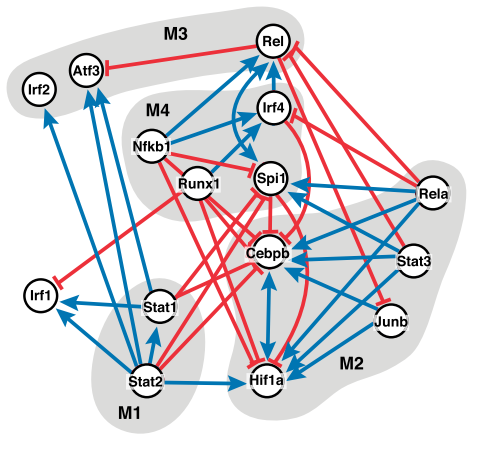
\includegraphics[width=0.5\linewidth]{slides/dixit_perturbseq_network.png}
  \caption{A regulatory network among transcription factors in mouse dendritic cells stimulated with lipopolysaccharide, inferred from a Perturb-seq screen. Blue arrows denote activation and red bar-headed arrows repression; grey regions mark modules M1--M4 of co-functional regulators. Reproduced from \citet{dixit2016}.}
  \label{fig:dixit}
\end{figure}

The readout in these experiments is almost always RNA. Protein levels can be measured for far fewer genes, and some regulation acts on translation or on splicing (Section~\ref{sec:te_ir}), so RNA is not an ideal readout, but it is the one we can measure most completely. Inferring a causal GRN remains hard even with perturbation data. Of the roughly 20{,}000 human protein-coding genes perhaps 8{,}000 are expressed in a given cell type, so the GRN is in principle an $8000\times 8000$ matrix of regulatory effects.

An older strategy reduces the number of parameters in two steps. Genes are first grouped into \emph{modules}, clusters of co-expressed genes, by clustering or by a matrix factorization such as non-negative matrix factorization (Chapter 8) that lets modules share genes. A network is then inferred between modules, or from regulators to modules, rather than between individual genes. Module networks~\citep{segal2003} learned regulators of yeast modules with probabilistic graphical models from observational expression data. \citet{mostafavi2018} applied a similar approach to RNA-seq from the aging human brain, inferring a network of a few tens of modules and linking some of them to amyloid and tau pathology and to cognitive decline. Bayesian network learning of this kind has become less common as perturbation data have grown.

\subsection{Protein-protein interaction networks}

To many biologists ``network'' means a \emph{protein-protein interaction} (PPI) network. The nodes are proteins and an undirected edge means that the two proteins physically bind. Proteins often act in complexes: RNA polymerase II, for example, transcribes DNA to RNA together with a large set of general transcription factors and the Mediator complex, all physically associated with it. Experimental methods usually start from one protein and find its partners, so interaction maps are assembled from many labor-intensive experiments. The results are collected in databases, of which the largest are BioGRID~\citep{stark2006} and STRING~\citep{szklarczyk2019}. STRING also includes predicted functional associations, for example from co-expression and text mining, not only physical binding.

PPI networks are best thought of as having a high false negative rate and a modest false positive rate. An edge in a curated database usually reflects a real interaction, but many true interactions are missing because nobody has tested them, and well-studied proteins have more recorded partners than less-studied ones. Figure~\ref{fig:scz} shows an example network built around genes associated with schizophrenia, which combined known interactions with several hundred newly predicted ones~\citep{ganapathiraju2016}.

\begin{figure}[tbp]
  \centering
  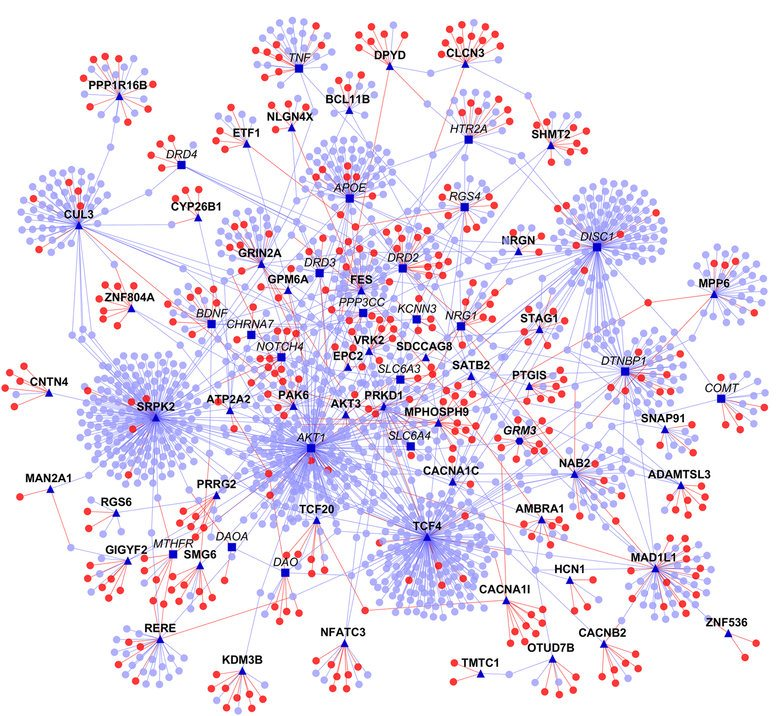
\includegraphics[width=0.65\linewidth]{slides/schizophrenia_interactome.png}
  \caption{A protein-protein interaction network centered on genes associated with schizophrenia (labelled nodes). Known interactions are combined with interactions predicted computationally. Reproduced from \citet{ganapathiraju2016}.}
  \label{fig:scz}
\end{figure}

\paragraph{Yeast two-hybrid screens.} The yeast two-hybrid (Y2H) assay~\citep{fields1989} tests whether two proteins X and Y bind. It uses the yeast transcription factor Gal4, which has two separable parts: a DNA binding domain (BD) that recognizes an upstream activating sequence (UAS), and an activation domain (AD) that recruits the transcriptional machinery. Neither part alone activates transcription. The ``bait'' protein X is fused to the BD and the ``prey'' protein Y to the AD, each expressed from its own plasmid. If X and Y interact, they bring the BD and AD together at the UAS and a reporter gene is transcribed, for example one needed for growth on a selective medium (Figure~\ref{fig:y2h}). Screening a bait against a library of prey reveals its binding partners.

\begin{figure}[tbp]
  \centering
  \begin{tikzpicture}[>=Stealth, every node/.style={font=\small}]
    % plasmids
    \draw[thick] (0,3.0) circle (0.55);
    \draw[line width=3pt, black] (0,3.0) ++(60:0.55) arc (60:110:0.55);
    \draw[line width=3pt, gray] (0,3.0) ++(115:0.55) arc (115:200:0.55);
    \node at (0.45,3.75) {X}; \node at (-0.95,2.95) {BD};
    \node at (0,2.15) {bait plasmid};
    \draw[thick] (4,3.0) circle (0.55);
    \draw[line width=3pt, black] (4,3.0) ++(60:0.55) arc (60:110:0.55);
    \draw[line width=3pt, gray] (4,3.0) ++(115:0.55) arc (115:200:0.55);
    \node at (4.45,3.75) {Y}; \node at (3.05,2.95) {AD};
    \node at (4,2.15) {prey plasmid};
    % fusion proteins
    \node[draw, fill=gray!50, minimum width=0.9cm, minimum height=0.45cm] (bd1) at (-0.3,1.1) {BD};
    \node[draw, ellipse, minimum width=0.7cm, minimum height=0.9cm] (x1) at (0.5,1.3) {X};
    \node[draw, ellipse, minimum width=0.7cm, minimum height=0.9cm] (y1) at (3.65,1.2) {Y};
    \node[draw, circle, fill=gray!50, minimum size=0.75cm] (ad1) at (4.4,0.95) {AD};
    \draw[->] (0,1.95) -- (0,1.75);
    \draw[->] (4,1.95) -- (4,1.75);
    % complex on DNA
    \draw[thick] (-1.2,-1) -- (7.5,-1);
    \node[draw, fill=white, minimum width=1.3cm, minimum height=0.45cm] (uas) at (-0.3,-1) {UAS};
    \node[draw, fill=white, minimum width=2.3cm, minimum height=0.45cm] (rep) at (5.6,-1) {reporter gene};
    \node[draw, fill=gray!50, minimum width=0.9cm, minimum height=0.45cm] (bd2) at (-0.3,-0.48) {BD};
    \node[draw, ellipse, minimum width=0.7cm, minimum height=0.9cm] (x2) at (0.55,-0.25) {X};
    \node[draw, ellipse, minimum width=0.7cm, minimum height=0.9cm] (y2) at (1.25,-0.25) {Y};
    \node[draw, circle, fill=gray!50, minimum size=0.75cm] (ad2) at (2.0,-0.55) {AD};
    \draw[->, thick] (4.45,-0.75) -- (4.45,-0.2) -- (6.6,-0.2) node[above, pos=0.5] {transcription};
    \draw[->, thick] (2.0,0.7) -- (2.0,0.1) node[midway, right] {if X binds Y};
  \end{tikzpicture}
  \caption{The yeast two-hybrid assay. The bait protein X is fused to the Gal4 DNA binding domain (BD) and the prey Y to the Gal4 activation domain (AD). If X and Y bind, the BD and AD are brought together at the upstream activating sequence (UAS) and the reporter gene is transcribed. After a slide figure of the assay~\citep{fields1989}.}
  \label{fig:y2h}
\end{figure}

\subsection{Genetic interaction networks}

Budding yeast, \textit{Saccharomyces cerevisiae}, is single-celled but, like us, a eukaryote, with a nucleus and much of the same core cellular machinery. A surprising amount of biology is conserved between yeast and humans; some of the proteins whose misfolding damages neurons in neurodegenerative disease are also toxic to yeast, for example. Yeast grows fast and is easy to manipulate genetically, which makes possible experiments that would be impractical in mammalian cells.

One such experiment maps \emph{genetic interactions}. A collection of yeast strains each lacking one of the roughly 6{,}000 genes (or carrying a weakened allele of an essential gene) can be crossed systematically to make double mutants, and the fitness of each double mutant measured from the size of its colony on an agar plate. \citet{costanzo2016} constructed and measured roughly 23 million double mutants. The colony size $C_{ij}$ of the double mutant lacking genes $i$ and $j$ is modelled as
\begin{equation}
  C_{ij} = f_{ij}\times t\times s_{ij}\times e,
\end{equation}
where $f_{ij}$ is the double-mutant fitness, $t$ is the growth time, $s_{ij}$ collects systematic experimental effects (such as position on the plate) and $e$ is noise. After estimating and removing $t$ and $s_{ij}$, the double-mutant fitness is compared with the product of the single-mutant fitnesses $f_i$ and $f_j$,
\begin{equation}
  f_{ij} = f_if_j + \epsilon_{ij}.
\end{equation}
The multiplicative model $f_if_j$ is the expected fitness if the two genes act independently, so that each deletion reduces growth by a fixed factor. The deviation $\epsilon_{ij}$ is the \emph{genetic interaction score}. A negative score, with the extreme case of synthetic lethality, means the double mutant is sicker than expected; this often happens when the two genes act in parallel pathways that can compensate for each other. A positive score means the double mutant is healthier than expected, as when both genes act in the same pathway or complex, so that losing one already disables it.

The matrix of scores $\epsilon_{ij}$ defines a weighted network over genes. More informative still is the \emph{profile} of each gene, its row of interaction scores with all other genes. Genes with similar profiles tend to have similar functions. Connecting genes whose profiles are correlated and laying out the resulting network gives the functional map of the yeast cell in Figure~\ref{fig:costanzo}, in which clusters correspond to cellular processes.

\begin{figure}[tbp]
  \centering
  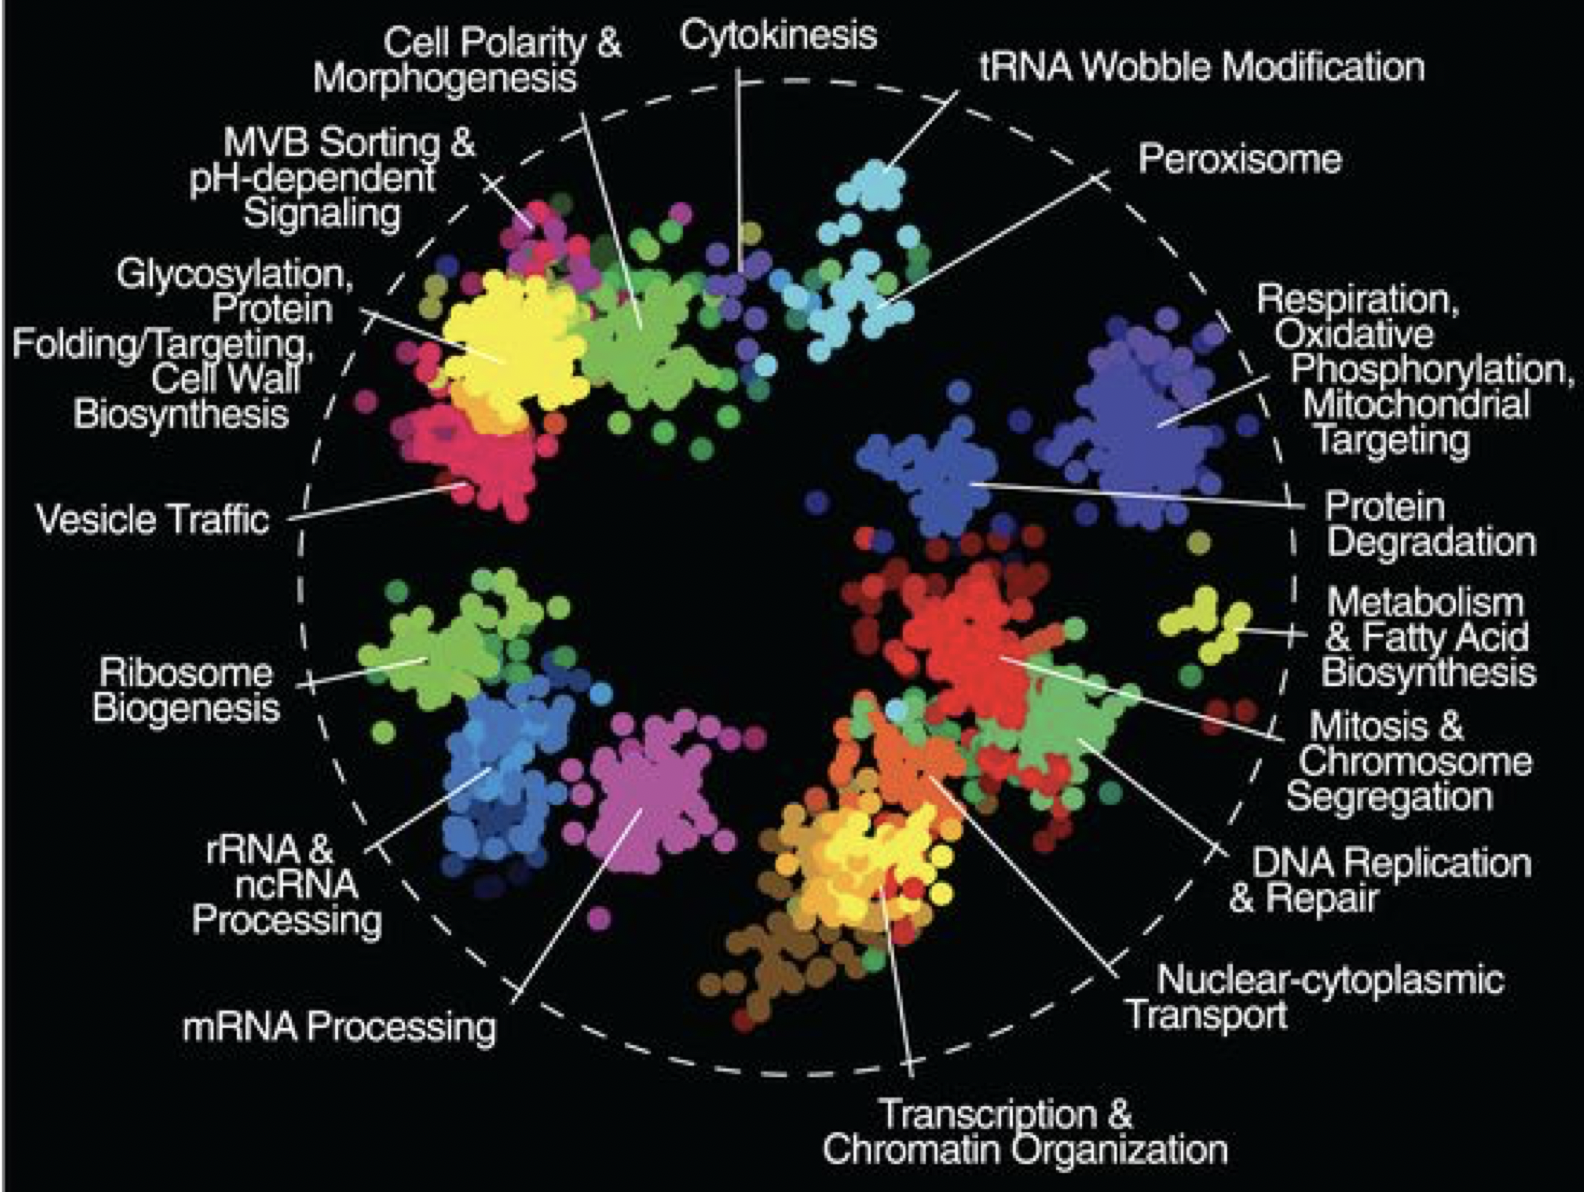
\includegraphics[width=0.75\linewidth]{slides/costanzo_functional_map.png}
  \caption{A global map of the yeast cell from genetic interaction profiles. Each dot is a gene; genes with similar genetic interaction profiles are placed near each other, and colored clusters are labelled by the biological process enriched in them. Reproduced from \citet{costanzo2016}.}
  \label{fig:costanzo}
\end{figure}

\subsection{Metabolic networks}

Metabolism is the set of chemical reactions by which a cell converts nutrients into energy and building blocks. A metabolic network has metabolites as nodes and reactions, catalyzed by enzymes, as edges; more precisely it is a bipartite graph between metabolites and reactions, or a hypergraph, since a reaction can take several substrates to several products. Pathways such as glycolysis, the citric acid cycle and fatty acid synthesis are paths through this network (Figure~\ref{fig:metabolic}). Curated metabolic pathways for many organisms are available in KEGG~\citep{kanehisa2000}.

\begin{figure}[tbp]
  \centering
  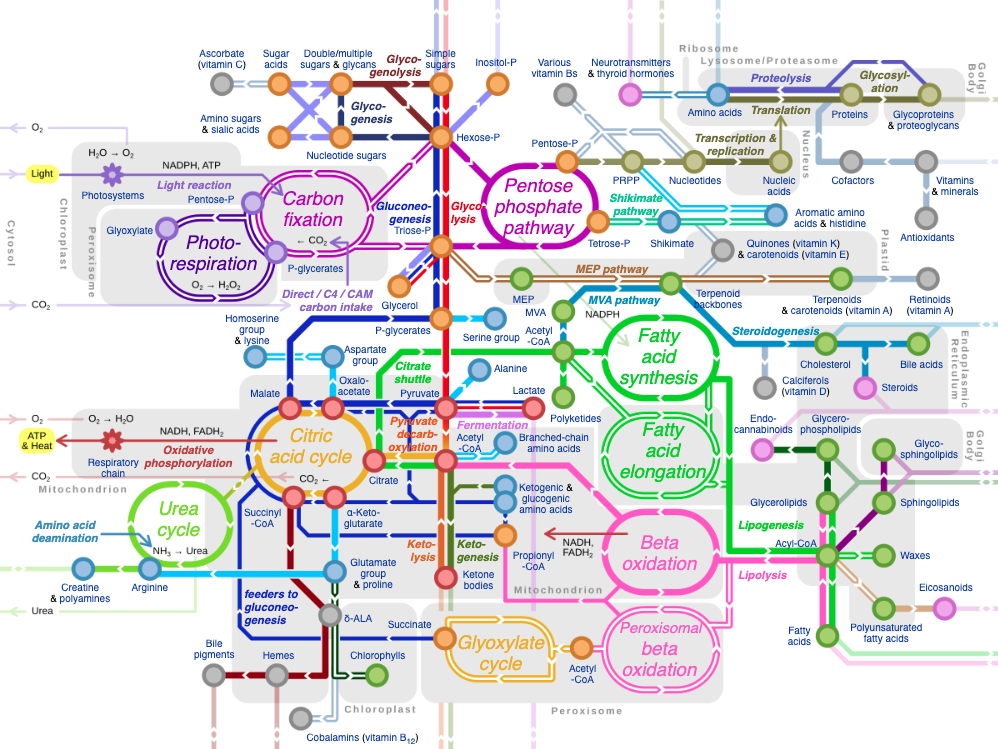
\includegraphics[width=0.8\linewidth]{slides/metabolic_metro_map.png}
  \caption{The core metabolic network drawn as a metro map. Stations are metabolites and lines are pathways. Image by Bert Chan, Hong Kong (``Metabolic Metro Map'', Wikimedia Commons).}
  \label{fig:metabolic}
\end{figure}

\subsection{Signaling networks}

Signaling networks transmit information from outside the cell to the nucleus. A ligand, such as a growth factor, binds a receptor on the cell surface, which triggers a cascade of protein modifications inside the cell, eventually changing the activity of TFs and hence gene expression (Figure~\ref{fig:signaling}). The most common modification is \emph{phosphorylation}: an enzyme called a \emph{kinase} transfers a phosphate group from ATP to a target protein, changing its shape and switching it on or off, and a \emph{phosphatase} removes the phosphate again. A cascade such as Ras$\to$Raf$\to$MEK$\to$ERK is a chain of kinases, each phosphorylating and activating the next. Signaling networks are central to cancer biology. Many oncogenes, such as \textit{RAS} and \textit{BRAF}, encode members of growth signaling pathways whose mutations make the pathway constitutively active, and many targeted cancer drugs are kinase inhibitors.

\begin{figure}[tbp]
  \centering
  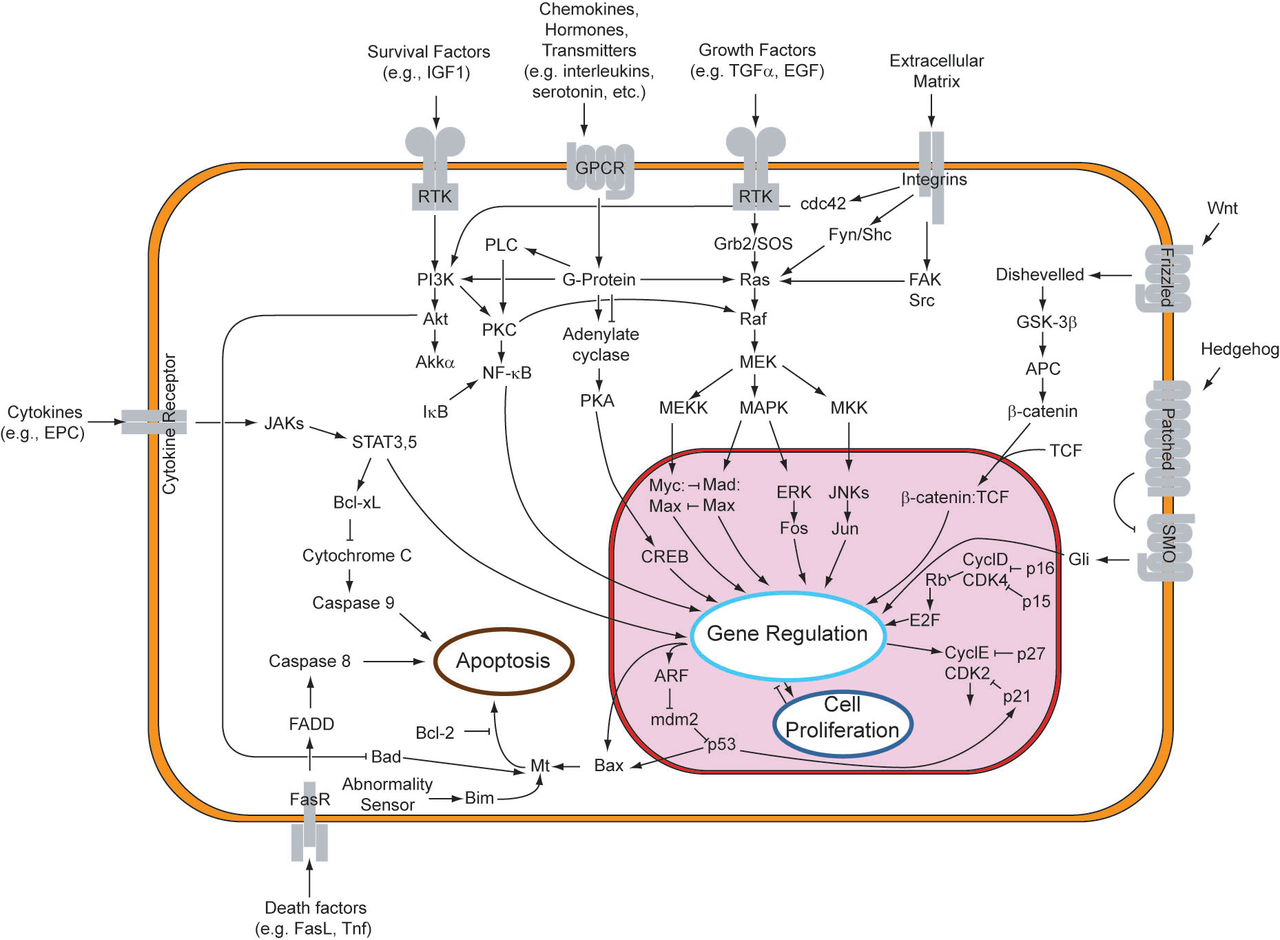
\includegraphics[width=0.85\linewidth]{slides/signaling_pathways.png}
  \caption{Major signaling pathways of a mammalian cell. Receptors at the cell membrane (orange) receive external signals such as growth factors, cytokines and death factors; cascades of protein interactions and phosphorylation in the cytoplasm relay the signal to gene regulation in the nucleus (pink), controlling proliferation and apoptosis. Source: Wikimedia Commons, signal transduction pathways diagram (source and license to be confirmed).}
  \label{fig:signaling}
\end{figure}

\subsection{Co-expression networks}

The networks above are measured, or curated from many experiments. A \emph{co-expression network} is instead inferred from expression data: nodes are genes, and an undirected edge means that the expression levels of the two genes are associated across samples. Genes regulated by the same factors will be correlated, so a co-expression network can be read as a network of co-regulation. The simplest construction connects pairs of genes whose correlation exceeds a threshold. The trouble is that correlation does not distinguish direct from indirect association. If gene $C$ regulates both $A$ and $B$, then $A$ and $B$ are correlated even though neither affects the other. The rest of the first half of this chapter develops a better approach based on partial correlation.

%======================================================================
\section{Networks of expression and splicing}
\label{sec:te_ir}
%======================================================================

Gene expression is not the only quantity a regulatory network can act on. Most human genes produce several \emph{isoforms}, transcripts that differ in which exons they include, through alternative splicing (Chapter 10). Splicing is controlled by \emph{splicing factors}, RNA-binding proteins that promote or repress the use of particular exons. \citet{saha2017} built co-expression networks from GTEx RNA-seq data~\citep{gtex2015} whose nodes are of two types. For each gene, the \emph{total expression} (TE) is the summed expression of all its isoforms. For each isoform, the \emph{isoform ratio} (IR) is its expression divided by the TE of its gene, so the IRs of a gene are non-negative and sum to one.

Table~\ref{tab:te_ir} shows why both are needed. A splicing regulator changes how a gene's transcripts are spliced. When it is abundant, most transcripts of a target gene are isoform 1; when it is scarce, more are isoform 2. The total expression of the target does not change, so a network built on TE alone cannot see this regulation, while the isoform ratios capture it.

\begin{table}[tbp]
  \centering
  \caption{Total expression (TE) and isoform ratios (IR) of a target gene with two isoforms, at high and low levels of a splicing regulator. Counts are numbers of transcripts. The regulator changes the isoform ratios but not the total expression. After an example in \citet{saha2017}.}
  \label{tab:te_ir}
  \begin{tabular}{lccccc}
    \toprule
    Splicing regulator & Isoform 1 & Isoform 2 & TE & IR$_1$ & IR$_2$ \\
    \midrule
    high & 4 & 1 & 5 & 0.8 & 0.2 \\
    low  & 2 & 3 & 5 & 0.4 & 0.6 \\
    \bottomrule
  \end{tabular}
\end{table}

The data for one tissue form a matrix $\mX\in\R^{N\times P}$, with $N$ samples (individuals) as rows and $P$ features as columns, the TE features of all genes followed by the IR features of all isoforms. The goal is a sparse undirected network over the $P$ features. The pipeline (Figure~\ref{fig:twn_pipeline}) computes the $P\times P$ sample covariance matrix, estimates a sparse inverse covariance, or precision, matrix from it with the graphical lasso, and reads the network off the non-zero entries of the precision matrix. The next two sections explain why the precision matrix is the right object and how the graphical lasso estimates it.

\begin{figure}[tbp]
  \centering
  \begin{tikzpicture}[>=Stealth, every node/.style={font=\small}]
    % data matrix
    \fill[blue!15] (0,0) rectangle (1.05,2.1);
    \fill[yellow!35] (1.05,0) rectangle (2.1,2.1);
    \draw (0,0) grid[step=0.35] (2.1,2.1);
    \node[above] at (0.525,2.1) {\footnotesize TE};
    \node[above] at (1.575,2.1) {\footnotesize IR};
    \node[left, rotate=90, anchor=south] at (-0.15,1.05) {samples ($N$)};
    \node[below] at (1.05,-0.05) {data $\mX$};
    \draw[->, thick] (2.4,1.05) -- (3.1,1.05);
    % covariance
    \begin{scope}[xshift=3.4cm]
      \fill[gray!20] (0,0) rectangle (2.1,2.1);
      \draw (0,0) grid[step=0.35] (2.1,2.1);
      \node[below, align=center] at (1.05,-0.05) {sample covariance\\$\hSigma$, $P\times P$};
    \end{scope}
    \draw[->, thick] (5.8,1.05) -- node[above, align=center] {\footnotesize graphical\\[-2pt]\footnotesize lasso} (7.1,1.05);
    % sparse precision
    \begin{scope}[xshift=7.4cm]
      \foreach \i/\j in {0/0,1/1,2/2,3/3,4/4,5/5,0/3,3/0,1/4,4/1,1/2,2/1,4/5,5/4}
        \fill[gray!45] (0.35*\i,2.1-0.35*\j-0.35) rectangle (0.35*\i+0.35,2.1-0.35*\j);
      \draw (0,0) grid[step=0.35] (2.1,2.1);
      \node[below, align=center] at (1.05,-0.05) {sparse precision\\$\hat\mTheta$, $P\times P$};
    \end{scope}
    \draw[->, thick] (9.8,1.05) -- (10.4,1.05);
    % network
    \begin{scope}[xshift=11.1cm, yshift=0.2cm, every node/.style={font=\footnotesize, inner sep=1.5pt}]
      \node[draw, circle, fill=blue!15] (t1) at (0,1.6) {1};
      \node[draw, circle, fill=blue!15] (t2) at (1.2,1.6) {2};
      \node[draw, circle, fill=blue!15] (t3) at (1.6,0.6) {3};
      \node[draw, rectangle, fill=yellow!35] (i4) at (0,0.3) {4};
      \node[draw, rectangle, fill=yellow!35] (i5) at (0.8,-0.2) {5};
      \node[draw, rectangle, fill=yellow!35] (i6) at (1.9,-0.4) {6};
      \draw (t1) -- (i4); \draw (t2) -- (i5); \draw (t2) -- (t3); \draw (i5) -- (i6);
      \node[below, font=\small] at (0.9,-0.6) {network};
    \end{scope}
  \end{tikzpicture}
  \caption{Inferring a network of total expression (TE, circles) and isoform ratio (IR, squares) features. The $N\times P$ data matrix gives a $P\times P$ sample covariance matrix; the graphical lasso estimates a sparse precision matrix whose non-zero off-diagonal entries (grey) are the edges of the network. After \citet{saha2017}.}
  \label{fig:twn_pipeline}
\end{figure}

%======================================================================
\section{Partial correlation}
\label{sec:partial_corr}
%======================================================================

\subsection{Direct and indirect association}

Consider five genes $A,B,C,D,E$. Suppose $C$ is a transcription factor that regulates both $A$ and $B$. Then $A$ and $B$ will be correlated across samples even if there is no direct relationship between them. We want an edge between $A$ and $B$ only if they remain associated after accounting for everything else that is measured. The \emph{partial correlation} of $A$ and $B$ given $C,D,E$ formalizes this. Let $x_{nA}$ be the expression of gene $A$ in sample $n$, and regress $x_A$ on the other genes,
\begin{equation}
  x_{nA} = \sum_{g\in\{C,D,E\}}\beta_gx_{ng} + \epsilon_{nA}, \qquad n=1,\dots,N.
\end{equation}
Fitting by ordinary least squares (Chapter 1) gives $\hat\vb$ and residuals $\hat\epsilon_{nA}=x_{nA}-\sum_g\hat\beta_gx_{ng}$, the part of $x_A$ that $C,D,E$ cannot explain. Doing the same for $B$ gives residuals $\hat\epsilon_{nB}$. The sample partial correlation is the correlation of the residuals,
\begin{equation}
  \cor(A,B\mid C,D,E) = \cor\left(\hat\epsilon_A,\hat\epsilon_B\right).
\end{equation}
If $C$ alone explains the association between $A$ and $B$, the residuals are uncorrelated and the partial correlation is near zero.

Running two regressions for each of the $P(P-1)/2$ pairs of genes would be expensive. It turns out that all partial correlations can be read off a single matrix, the inverse of the covariance matrix.

\subsection{Partial correlations from the precision matrix}

Let $\vx\in\R^P$ be a random vector, one sample of the expression of $P$ genes, with $\vx\sim\Normal(\mathbf{0},\mSigma)$. The data are centered so the mean is zero. $\mSigma\in\R^{P\times P}$ is the covariance matrix and $\mTheta=\mSigma^{-1}\in\R^{P\times P}$ is the \emph{precision matrix}, with entries $\theta_{ij}$. Split the coordinates into a block $1=\{A,B\}$ of size 2 and a block $2$ of the remaining $P-2$ genes, and partition
\begin{equation}
  \vx = \begin{pmatrix}\vx_1\\ \vx_2\end{pmatrix},\qquad
  \mSigma = \begin{pmatrix}\mSigma_{11} & \mSigma_{12}\\ \mSigma_{21} & \mSigma_{22}\end{pmatrix},\qquad
  \mTheta = \begin{pmatrix}\mTheta_{11} & \mTheta_{12}\\ \mTheta_{21} & \mTheta_{22}\end{pmatrix},
\end{equation}
where $\mSigma_{11},\mTheta_{11}$ are $2\times 2$, $\mSigma_{12},\mTheta_{12}$ are $2\times(P-2)$ and $\mSigma_{22},\mTheta_{22}$ are $(P-2)\times(P-2)$.

The population version of regressing $\vx_1$ on $\vx_2$ uses the coefficients that minimize expected squared error, $\mathbf{B}=\mSigma_{12}\mSigma_{22}^{-1}$, a $2\times(P-2)$ matrix. (This is the population analogue of $(\mX^\top\mX)^{-1}\mX^\top\vy$: setting the derivative of $\E\|\vx_1-\mathbf{B}\vx_2\|^2$ to zero gives $\mathbf{B}\mSigma_{22}=\mSigma_{12}$.) The residual $\veps_1=\vx_1-\mathbf{B}\vx_2$ has covariance
\begin{align}
  \Cov(\veps_1) &= \mSigma_{11} - \mathbf{B}\mSigma_{21} - \mSigma_{12}\mathbf{B}^\top + \mathbf{B}\mSigma_{22}\mathbf{B}^\top \nonumber\\
  &= \mSigma_{11} - \mSigma_{12}\mSigma_{22}^{-1}\mSigma_{21},
\end{align}
the \emph{Schur complement} of $\mSigma_{22}$ in $\mSigma$. For Gaussian $\vx$ this is also the covariance of the conditional distribution of $\vx_1$ given $\vx_2$, which is $\Normal(\mathbf{B}\vx_2,\,\mSigma_{11}-\mSigma_{12}\mSigma_{22}^{-1}\mSigma_{21})$.

The block matrix inversion formula states that the top-left block of the inverse of a partitioned matrix is the inverse of this Schur complement,
\begin{equation}
  \mTheta_{11} = \left(\mSigma_{11}-\mSigma_{12}\mSigma_{22}^{-1}\mSigma_{21}\right)^{-1}.
\end{equation}
(To check, multiply $\mSigma$ by $\mTheta$ and use $\mTheta_{21}=-\mSigma_{22}^{-1}\mSigma_{21}\mTheta_{11}$, which follows from the bottom-left block of $\mSigma\mTheta=\mI$.) So $\Cov(\veps_1)=\mTheta_{11}^{-1}$. Writing out the inverse of the $2\times2$ block,
\begin{equation}
  \mTheta_{11}^{-1} = \begin{pmatrix}\theta_{AA} & \theta_{AB}\\ \theta_{AB} & \theta_{BB}\end{pmatrix}^{-1}
  = \frac{1}{\theta_{AA}\theta_{BB}-\theta_{AB}^2}\begin{pmatrix}\theta_{BB} & -\theta_{AB}\\ -\theta_{AB} & \theta_{AA}\end{pmatrix}.
\end{equation}
The correlation of the two residuals is the off-diagonal entry divided by the square root of the product of the diagonal entries; the determinant cancels and
\begin{equation}
  \rho_{AB\mid\text{rest}} = \cor(\epsilon_A,\epsilon_B) = -\frac{\theta_{AB}}{\sqrt{\theta_{AA}\theta_{BB}}}.
  \label{eq:partial_corr}
\end{equation}
The partial correlation of every pair of variables, given all the others, is the corresponding entry of the precision matrix, rescaled by the diagonal and with its sign flipped. In particular, $\rho_{AB\mid\text{rest}}=0$ exactly when $\theta_{AB}=0$.

The same block formula with block $1=\{A\}$ alone relates the precision matrix to the regression of one gene on all the others. Using $\mTheta_{21}=-\mSigma_{22}^{-1}\mSigma_{21}\mTheta_{11}$ with $\mTheta_{11}=\theta_{AA}$ a scalar, the regression coefficients are $\mSigma_{22}^{-1}\mSigma_{21}=-\mTheta_{21}/\theta_{AA}$, that is
\begin{equation}
  \beta_{Aj} = -\frac{\theta_{Aj}}{\theta_{AA}}, \qquad \Var(\epsilon_A) = \frac{1}{\theta_{AA}}.
\end{equation}
Gene $j$ has a non-zero coefficient in the regression of $A$ on all other genes exactly when $\theta_{Aj}\neq 0$. This suggests estimating the network by a sparse (lasso) regression of each gene on all the others, \emph{neighbourhood selection}~\citep{meinshausen2006}.

\subsection{Conditional independence and Gaussian graphical models}

For Gaussian $\vx$, the conditional distribution of $(x_A,x_B)$ given the other genes is Gaussian with covariance $\mTheta_{11}^{-1}$. A bivariate Gaussian has independent components if and only if its covariance is diagonal, so
\begin{equation}
  \rho_{AB\mid\text{rest}}=0 \iff \theta_{AB}=0 \iff x_A\indep x_B\mid \vx_{\text{rest}} .
\end{equation}
The same conclusion follows from the density. Up to a constant, $\log p(\vx) = \frac12\log|\mTheta| - \frac12\sum_{i,j}\theta_{ij}x_ix_j$, so if $\theta_{AB}=0$ no term couples $x_A$ and $x_B$ and the density factorizes into a part involving $x_A$ and a part involving $x_B$, given the rest. A Gaussian distribution together with the graph whose edges are the non-zero off-diagonal entries of $\mTheta$ is a \emph{Gaussian graphical model}, or Gaussian Markov random field. Missing edges are conditional independences. The equivalence between zero partial correlation and conditional independence is special to the Gaussian; for other distributions zero partial correlation only means the absence of linear association given the other variables.

The precision matrix contains the direct associations; the covariance matrix contains direct and indirect associations mixed together. In the five-gene example above, if $A$ is directly linked only to $C$ and $B$ only to $E$, then $\theta_{AB}=0$ and the graph has no $A$--$B$ edge, though $\Sigma_{AB}$ may be far from zero if $C$ and $E$ are themselves associated.

Figure~\ref{fig:partial_corr} illustrates this with a simulated network of eight genes: a hub (gene 1 linked to genes 2, 3 and 4), a chain $5-6-7$, and an isolated gene 8. The sample correlation matrix is dense, because genes 2, 3 and 4 are correlated through gene 1 and genes 5 and 7 through gene 6. With $N=100$ samples genes 5 and 7 have sample correlation $\corrFiveSeven$ but sample partial correlation $\pcorFiveSeven$. The partial correlations computed from the inverse of the sample covariance recover the structure, but with noise everywhere; the graphical lasso (Section~\ref{sec:glasso}) sets most of the spurious entries exactly to zero.

\begin{figure}[tbp]
  \centering
  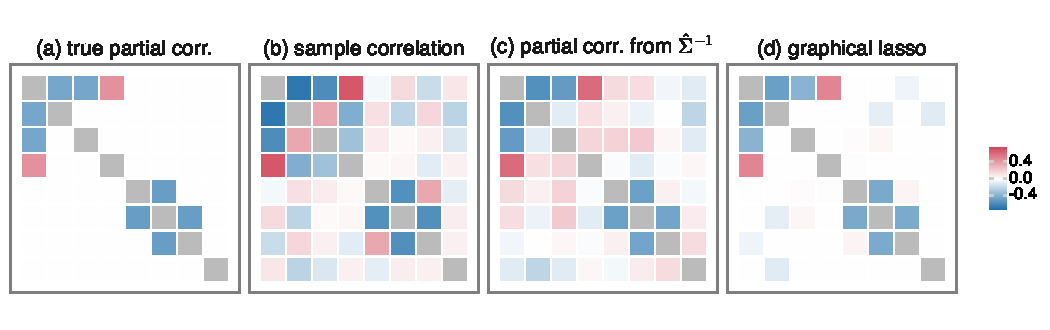
\includegraphics[width=\linewidth]{partial_correlation.pdf}
  \caption{Correlation and partial correlation for eight simulated genes ($N=100$ samples). (a) True partial correlations $-\theta_{ij}/\sqrt{\theta_{ii}\theta_{jj}}$: gene 1 is a hub linked to genes 2--4 and genes 5--6--7 form a chain. (b) The sample correlation matrix is dense, because of indirect associations. (c) Partial correlations from the inverse sample covariance $\hSigma^{-1}$ recover the structure, with noise. (d) Partial correlations from the graphical lasso with $\lambda=0.1$, which are exactly zero for most non-edges. Diagonal entries are grey.}
  \label{fig:partial_corr}
\end{figure}

%======================================================================
\section{The graphical lasso}
\label{sec:glasso}
%======================================================================

\subsection{Gaussian likelihood in terms of the precision matrix}

Let $\vx_n\in\R^P$, $n=1,\dots,N$, be the centered expression vectors of $N$ samples, assumed independent and identically distributed as $\vx_n\sim\Normal(\mathbf{0},\mTheta^{-1})$ with unknown $P\times P$ precision matrix $\mTheta$. The Gaussian density is $p(\vx_n)=(2\pi)^{-P/2}|\mTheta|^{1/2}\exp(-\frac12\vx_n^\top\mTheta\vx_n)$, using $|\mSigma|^{-1/2}=|\mTheta^{-1}|^{-1/2}=|\mTheta|^{1/2}$. The log likelihood is
\begin{equation}
  \log L(\mTheta) = \sum_{n=1}^N\left(\frac12\log|\mTheta| - \frac12\vx_n^\top\mTheta\vx_n\right) + \text{const}.
\end{equation}
A scalar equals its own trace, and the trace is invariant to cyclic permutations, so $\vx_n^\top\mTheta\vx_n=\tr(\vx_n^\top\mTheta\vx_n)=\tr(\mTheta\vx_n\vx_n^\top)$. Summing over $n$ and using linearity of the trace,
\begin{equation}
  \sum_{n=1}^N\vx_n^\top\mTheta\vx_n = \tr\Big(\mTheta\sum_{n=1}^N\vx_n\vx_n^\top\Big) = N\tr(\mTheta\hSigma),
  \qquad \hSigma = \frac1N\sum_{n=1}^N\vx_n\vx_n^\top = \frac1N\mX^\top\mX,
\end{equation}
where $\hSigma\in\R^{P\times P}$ is the sample covariance matrix. Therefore
\begin{equation}
  \log L(\mTheta) = \frac N2\left(\log|\mTheta| - \tr(\mTheta\hSigma)\right) + \text{const}.
  \label{eq:gauss_loglik}
\end{equation}
The data enter only through $\hSigma$, a sufficient statistic.

To maximize, we need two matrix derivatives: $\partial\log|\mTheta|/\partial\mTheta=\mTheta^{-1}$ for symmetric positive definite $\mTheta$, and $\partial\tr(\mTheta\hSigma)/\partial\mTheta=\hSigma$. Setting the gradient of~\eqref{eq:gauss_loglik} to zero gives $\mTheta^{-1}=\hSigma$, so the maximum likelihood estimate is $\hat\mTheta=\hSigma^{-1}$, as used in Figure~\ref{fig:partial_corr}c. This estimate has two problems for genomic data. First, $\hSigma=\frac1N\mX^\top\mX$ has rank at most $N$ (at most $N-1$ once the data are centered), so when $N\le P$ it is singular and the inverse does not exist; with $P=10{,}000$ genes we would need more than 10{,}000 samples. Second, even when $N>P$, $\hSigma^{-1}$ is noisy and dense: no entry is exactly zero, so it does not give a network.

\subsection{The L1-penalized objective}

The graphical lasso~\citep{friedman2008,yuan2007,banerjee2008} applies the idea of the lasso (Chapter 1) to the precision matrix. Multiplying the log likelihood~\eqref{eq:gauss_loglik} by $-2/N$ to obtain a loss, and adding an L1 penalty on the entries of $\mTheta$,
\begin{equation}
  \hat\mTheta = \argmin_{\mTheta\succ 0}\; -\log|\mTheta| + \tr(\mTheta\hSigma) + \lambda\|\mTheta\|_1,
  \qquad \|\mTheta\|_1=\sum_{i,j}|\theta_{ij}|,
  \label{eq:glasso}
\end{equation}
where $\mTheta\succ0$ restricts $\mTheta$ to symmetric positive definite matrices and $\lambda\ge0$ is the regularization strength. Many implementations penalize only the off-diagonal entries, since the diagonal is always non-zero and does not correspond to edges. As in the lasso, the L1 penalty sets many entries of $\hat\mTheta$ exactly to zero, giving a sparse network, and for $\lambda>0$ the solution exists even when $\hSigma$ is singular.

The problem is convex. The function $-\log|\mTheta|$ is convex on positive definite matrices, $\tr(\mTheta\hSigma)$ is linear and $\|\mTheta\|_1$ is convex, so any local minimum is the global minimum. Whatever initialization or algorithm is used, a correct solver arrives at the same answer, unlike many of the non-convex problems in this book.

\subsection{A block coordinate descent algorithm}

The minimizer of~\eqref{eq:glasso} satisfies the subgradient condition
\begin{equation}
  \mTheta^{-1} - \hSigma - \lambda\mGamma = \mathbf{0},
  \label{eq:glasso_kkt}
\end{equation}
where $\mGamma$ is a $P\times P$ matrix with $\gamma_{ij}=\operatorname{sign}(\theta_{ij})$ if $\theta_{ij}\neq0$ and $\gamma_{ij}\in[-1,1]$ if $\theta_{ij}=0$. Let $\mathbf{W}=\mTheta^{-1}$ be the current estimate of the covariance. Condition~\eqref{eq:glasso_kkt} says $|w_{ij}-\hat\sigma_{ij}|\le\lambda$, with equality wherever $\theta_{ij}\neq0$: the estimated covariance may differ from the sample covariance by at most $\lambda$ in each entry.

\citet{friedman2008} solve~\eqref{eq:glasso_kkt} one row and column at a time. Partition $\mathbf{W}$, $\hSigma$, $\mTheta$ and $\mGamma$ with the last row and column separated, for example
\begin{equation}
  \mathbf{W} = \begin{pmatrix}\mathbf{W}_{11} & \mathbf{w}_{12}\\ \mathbf{w}_{12}^\top & w_{22}\end{pmatrix},
\end{equation}
where $\mathbf{W}_{11}$ is $(P-1)\times(P-1)$, $\mathbf{w}_{12}\in\R^{P-1}$ and $w_{22}$ is a scalar. The upper-right block of~\eqref{eq:glasso_kkt} is $\mathbf{w}_{12}-\hat{\boldsymbol\sigma}_{12}-\lambda\boldsymbol\gamma_{12}=\mathbf{0}$. The upper-right block of $\mathbf{W}\mTheta=\mI$ is $\mathbf{W}_{11}\boldsymbol\theta_{12}+\mathbf{w}_{12}\theta_{22}=\mathbf{0}$, so $\mathbf{w}_{12}=\mathbf{W}_{11}\vb$ with $\vb=-\boldsymbol\theta_{12}/\theta_{22}\in\R^{P-1}$. Because $\theta_{22}>0$, $\vb$ and $\boldsymbol\theta_{12}$ have opposite signs and the same zeros, so $\boldsymbol\gamma_{12}=-\boldsymbol\nu$ with $\nu_j\in\operatorname{sign}(\beta_j)$. Substituting,
\begin{equation}
  \mathbf{W}_{11}\vb - \hat{\boldsymbol\sigma}_{12} + \lambda\boldsymbol\nu = \mathbf{0}.
\end{equation}
This is the subgradient condition of
\begin{equation}
  \min_{\vb}\;\frac12\vb^\top\mathbf{W}_{11}\vb - \vb^\top\hat{\boldsymbol\sigma}_{12} + \lambda\|\vb\|_1,
\end{equation}
which is a lasso regression: with $\mathbf{W}_{11}=\hSigma_{11}$ it is exactly the lasso regression of the last variable on the others, written in terms of the covariances $\mX^\top\mX/N$ and $\mX^\top\vy/N$. It can be solved by coordinate descent, cycling over $j$ and updating
\begin{equation}
  \beta_j \leftarrow \frac{\mathcal{S}\big(\hat\sigma_{12,j}-\sum_{k\neq j}(\mathbf{W}_{11})_{kj}\beta_k,\;\lambda\big)}{(\mathbf{W}_{11})_{jj}},
\end{equation}
where $\mathcal{S}(u,\lambda)=\operatorname{sign}(u)\max(|u|-\lambda,0)$ is the soft-thresholding operator from Chapter 1. The algorithm initializes $\mathbf{W}=\hSigma+\lambda\mI$ (the diagonal of~\eqref{eq:glasso_kkt} when the diagonal is penalized), then cycles over the columns: each column in turn is moved to the last position, its lasso problem solved, and $\mathbf{w}_{12}=\mathbf{W}_{11}\hat\vb$ filled in. On convergence, $\mTheta$ is recovered from $\theta_{22}=1/(w_{22}-\mathbf{w}_{12}^\top\hat\vb)$ and $\boldsymbol\theta_{12}=-\hat\vb\,\theta_{22}$. Each column's lasso is the neighbourhood regression of the previous section, coupled across columns through $\mathbf{W}$. \citet{mazumder2012} analyze this algorithm and alternatives, including solving the primal problem directly; proximal gradient methods also work.

\subsection{\texorpdfstring{Choosing $\lambda$}{Choosing lambda}}

As in regression, $\lambda$ trades off fit and sparsity. Cross-validation applies even though there is no response variable: the Gaussian model assigns a likelihood to held-out samples. For each fold, fit $\hat\mTheta$ on the training samples and evaluate~\eqref{eq:gauss_loglik} with $\hat\mTheta$ and the held-out sample covariance. Figure~\ref{fig:glasso_path} shows the regularization path and the cross-validated log likelihood for $P=40$ simulated genes with 25 true edges and only $N=30$ samples, so that $\hSigma$ has rank $\pathRank$ and cannot be inverted. Small $\lambda$ overfits and gives a poor held-out likelihood. The cross-validated optimum, $\lambda=\pathBestLambda$, keeps $\pathBestEdges$ edges, $\pathBestTrue$ of them true. Cross-validation optimizes prediction, and the predictive optimum typically includes some false positive edges; if the network itself is the goal, a larger $\lambda$ or a stability-based criterion may be preferable.

\begin{figure}[tbp]
  \centering
  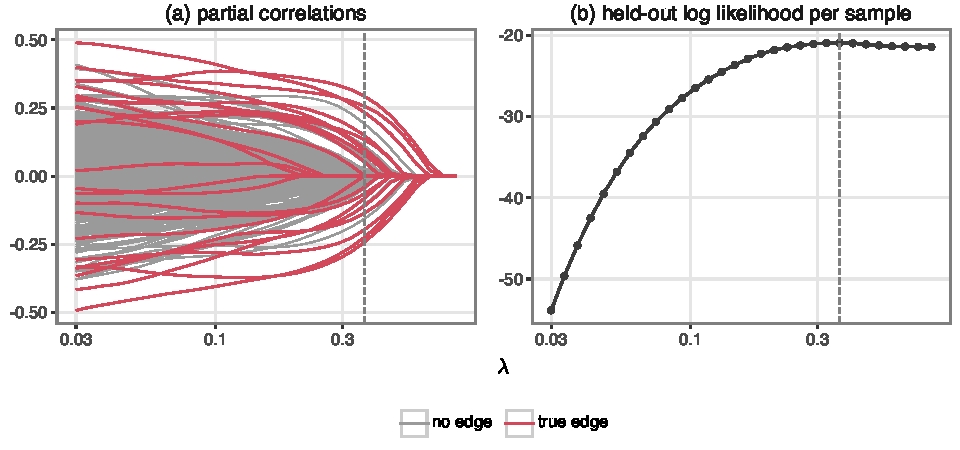
\includegraphics[width=0.95\linewidth]{glasso_path.pdf}
  \caption{The graphical lasso on simulated data with $P=40$ genes, 25 true edges and $N=30$ samples. (a) Partial correlations as a function of $\lambda$, for true edges (red) and non-edges (grey); every partial correlation reaches zero for large enough $\lambda$, and true edges tend to persist longest. (b) Five-fold cross-validated Gaussian log likelihood per held-out sample. The dashed line marks the $\lambda$ that maximizes it.}
  \label{fig:glasso_path}
\end{figure}

\subsection{Using the graphical lasso on expression data}

Several practical points matter when applying the graphical lasso to gene expression.
\begin{itemize}
  \item The model is Gaussian. Count data should be normalized and log-transformed, or each gene's values replaced by Gaussian quantiles of its ranks, an approach formalized by the nonparanormal~\citep{liu2009}.
  \item Hidden confounders, such as batch, RNA quality or cell-type composition, affect many genes at once and induce dense correlations. They are commonly removed first by regressing out known covariates and leading principal components or factors (Chapter 8).
  \item The network is undirected. An edge means a conditional association, not a causal or regulatory direction.
  \item Penalties need not be equal. With TE and IR features, for example, one could use different values of $\lambda$ for TE--TE, TE--IR and IR--IR entries. The isoform ratios of a gene sum to one, so one of them is a linear function of the others; dropping one ratio per gene avoids an exactly singular covariance.
\end{itemize}

\subsection{Network motifs}

Recurring local patterns in a network are called \emph{network motifs}, a term borrowed from the sequence motifs bound by TFs. In a network of TE and IR features, a node connected to many others is a \emph{hub}, and the type of hub suggests a mechanism (Figure~\ref{fig:hubs}). A TE node linked to many TE nodes could be a TF that regulates the expression of many targets. A TE node linked to many IR nodes could be a splicing factor, whose expression level controls the splicing of many targets. An IR node of a gene linked to many TE nodes suggests a TF with several isoforms that differ in their regulatory activity. An IR node linked to many IR nodes suggests alternative splicing of a splicing factor. Splicing factors often regulate the splicing of their own transcripts, a form of autoregulation that complicates the interpretation of such networks.

\begin{figure}[tbp]
  \centering
  \begin{tikzpicture}[every node/.style={font=\footnotesize},
      te/.style={draw, ellipse, fill=blue!15, minimum width=0.75cm, minimum height=0.45cm, inner sep=1pt},
      ir/.style={draw, rectangle, rounded corners=1pt, fill=yellow!35, minimum width=0.6cm, minimum height=0.45cm, inner sep=1pt}]
    \foreach \hx/\htype/\ltype/\lab/\mech in {0/te/te/TE--TE hub/{TF?}, 3.4/te/ir/TE--IR hub/{splicing factor}, 6.8/ir/te/IR--TE hub/{alternative splicing\\of a TF}, 10.2/ir/ir/IR--IR hub/{alternative splicing\\of a splicing factor}} {
      \node[\htype, thick] (h) at (\hx,0) {hub};
      \foreach \a in {90,162,234,306,18} {
        \node[\ltype] (l\a) at ($(\hx,0)+(\a:1.15)$) {};
        \draw (h) -- (l\a);
      }
      \node[below, font=\small] at (\hx,-1.45) {\lab};
      \node[below, align=center] at (\hx,-1.85) {\mech};
    }
  \end{tikzpicture}
  \caption{Four kinds of hub in a network of total expression (TE, ellipses) and isoform ratio (IR, rectangles) features, and the mechanism each suggests. After \citet{saha2017}.}
  \label{fig:hubs}
\end{figure}

%======================================================================
\section{Tissue-specific networks}
\label{sec:gtex}
%======================================================================

\subsection{The GTEx project}

The Genotype-Tissue Expression (GTEx) project~\citep{gtex2013,gtex2015,gtex2020} collected many tissues from postmortem donors, eventually close to a thousand individuals and around 50 tissues, and measured gene expression in each by RNA-seq and the donors' genotypes by sequencing or genotyping arrays. Its main aim was mapping genetic variants that affect expression (Chapter 12), but it is also a resource for asking how gene networks differ between tissues. Different tissues express different genes and are regulated differently, so a network estimated from one tissue need not hold in another.

Sample sizes per tissue are modest. In the early releases most tissues had tens of samples and the best represented, such as whole blood and skeletal muscle, had one to two hundred. Estimating a $10{,}000\times10{,}000$ precision matrix from 168 blood samples, for example, is a very high-dimensional problem. Some tissues are similar to each other, however. GTEx sampled more than ten brain regions, which in retrospect have similar expression profiles; arteries from different sites resemble each other, as do stomach and colon. Hierarchical clustering (Chapter 5) of the tissues' average expression profiles makes these similarities explicit (Figure~\ref{fig:gtex_dendrogram}). Information can therefore be shared between related tissues when estimating their networks. Pooling samples from similar tissues is the crude version of this; \citet{pierson2015} proposed a more principled one. Figure~\ref{fig:coronary} shows part of a network they inferred for coronary artery.

\begin{figure}[tbp]
  \centering
  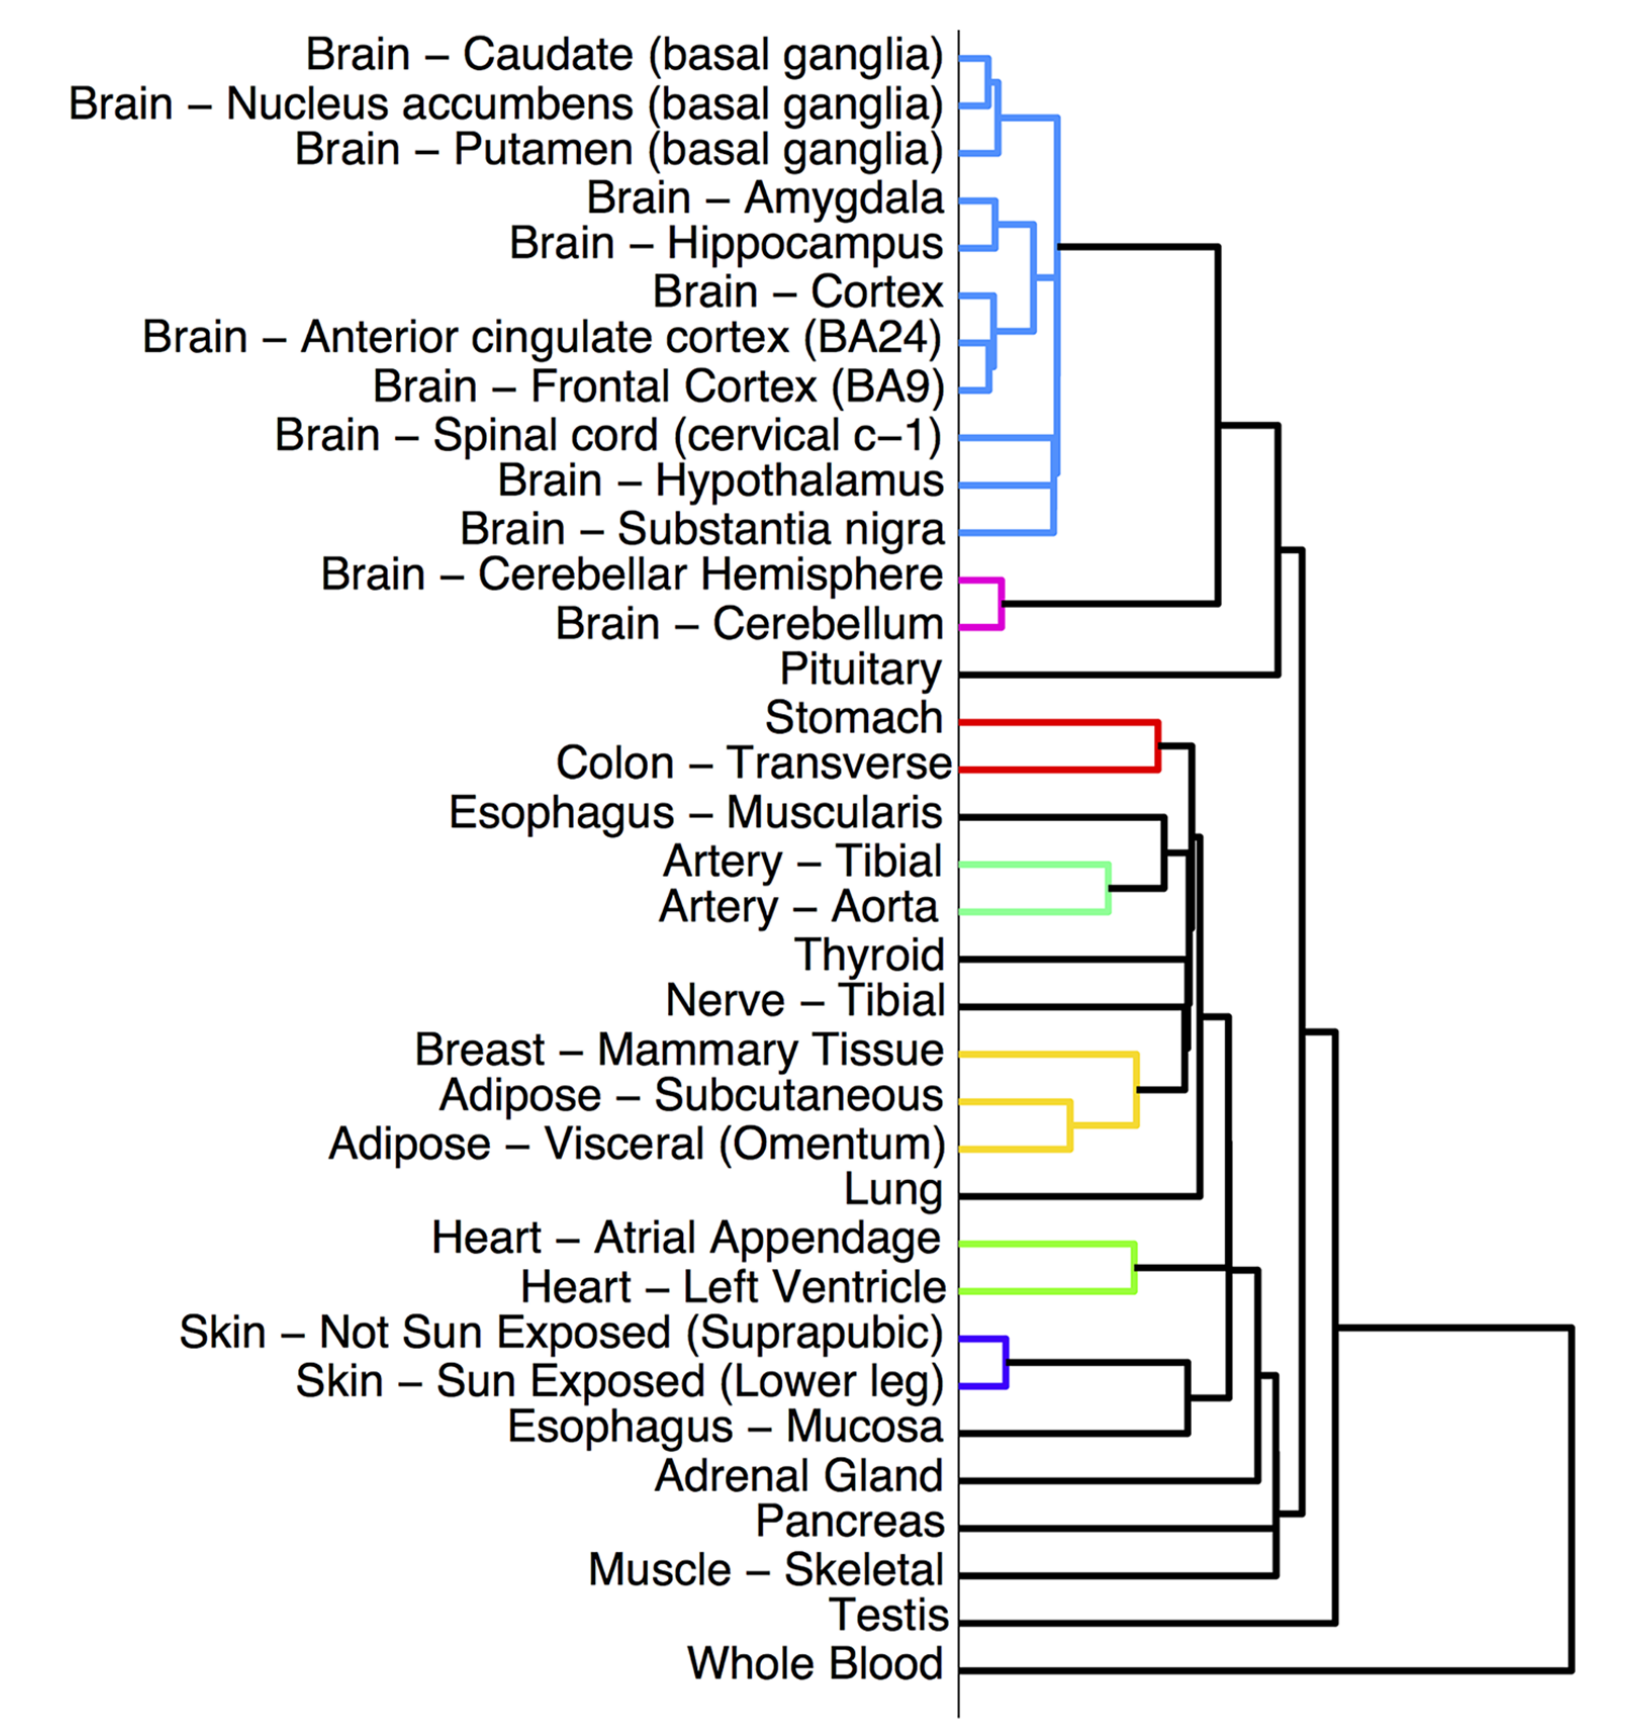
\includegraphics[width=0.6\linewidth]{slides/gtex_tissue_dendrogram.png}
  \caption{Hierarchical clustering of GTEx tissues by their average expression profiles. Brain regions form one tight cluster; arteries, the two adipose depots, the two heart samples and the two skin samples each cluster together. Reproduced from \citet{pierson2015}.}
  \label{fig:gtex_dendrogram}
\end{figure}

\begin{figure}[tbp]
  \centering
  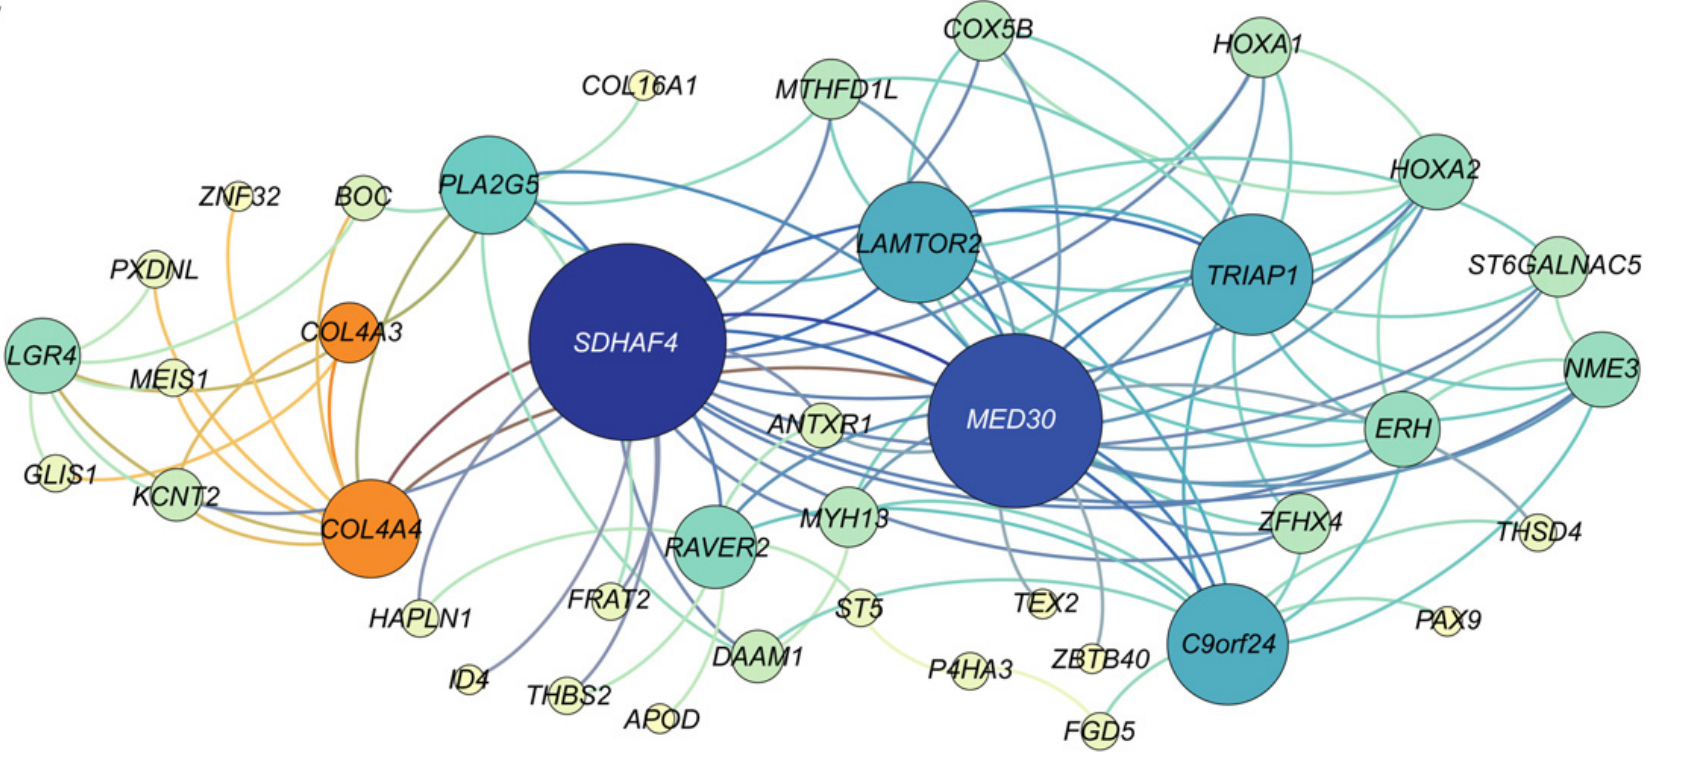
\includegraphics[width=0.8\linewidth]{slides/pierson_coronary_network.png}
  \caption{Part of a co-expression network inferred for GTEx coronary artery. Node size reflects the number of connections. Reproduced from \citet{pierson2015}.}
  \label{fig:coronary}
\end{figure}

\subsection{Sharing networks along a tissue hierarchy}

Let there be $K$ tissues, with $n^{(k)}$ samples and sample covariance $\hSigma^{(k)}\in\R^{P\times P}$ for tissue $k$. The tissue tree from hierarchical clustering is a rooted binary tree with the $K$ observed tissues as leaves, numbered $1,\dots,K$. A rooted binary tree with $K$ leaves has $K-1$ internal nodes, numbered $K+1,\dots,2K-1$ with the root last, and $2K-2$ edges, since every node except the root has exactly one parent. Each internal node can be thought of as an unobserved ``ancestral'' tissue. Give every node $k$ of the tree, leaf or internal, a precision matrix $\mTheta^{(k)}\in\R^{P\times P}$, and let $p(k)$ denote the parent of node $k$. \citet{pierson2015} estimate all $2K-1$ matrices jointly by maximizing
\begin{equation}
  \sum_{k=1}^{K}\frac{n^{(k)}}{2}\left(\log|\mTheta^{(k)}| - \tr\big(\mTheta^{(k)}\hSigma^{(k)}\big) - \lambda_s^{(k)}\|\mTheta^{(k)}\|_1\right)
  - \lambda_p\sum_{k=1}^{2K-2}\big\|\mTheta^{(k)}-\mTheta^{(p(k))}\big\|_2^2 ,
  \label{eq:gtex_objective}
\end{equation}
where $\|\cdot\|_2^2$ is the squared Frobenius norm, the sum of squared entries. The first sum is a graphical lasso objective for each observed tissue, weighted by its sample size, with tissue-specific sparsity penalties $\lambda_s^{(k)}$. The second sum runs over the $2K-2$ edges of the tree and penalizes the squared difference between the precision matrix of each node and that of its parent, with strength $\lambda_p\ge0$. With $\lambda_p=0$ the tissues are estimated independently. As $\lambda_p\to\infty$ all nodes are forced to share one network, which amounts to pooling. In between, each tissue's network is pulled toward those of the tissues near it in the tree. For a tree with $K=3$ leaves in which tissues 1 and 2 share parent 4, and 4 and 3 are children of the root 5, the four penalty terms are $\|\mTheta^{(1)}-\mTheta^{(4)}\|^2$, $\|\mTheta^{(2)}-\mTheta^{(4)}\|^2$, $\|\mTheta^{(4)}-\mTheta^{(5)}\|^2$ and $\|\mTheta^{(3)}-\mTheta^{(5)}\|^2$.

Figure~\ref{fig:tissue_tree} gives the intuition with three genes. Estimated separately, each tissue's network reflects its own small sample. An internal node's network is an average of its children: if both children have an $A$--$B$ edge, so does the parent, and if only one has an $A$--$C$ edge, the parent has a weaker one. Re-estimating each tissue with a pull toward its parent then shares edges between similar tissues.

\begin{figure}[tbp]
  \centering
  \begin{tikzpicture}[every node/.style={font=\scriptsize}]
    \newcommand{\abc}[6]{% x, y, color, A-B width, A-C width, B-C width (0pt = no edge)
      \begin{scope}[shift={(#1,#2)}]
        \node[draw, circle, fill=#3, inner sep=1pt, minimum size=0.36cm] (nA) at (-0.3,0) {A};
        \node[draw, circle, fill=#3, inner sep=1pt, minimum size=0.36cm] (nB) at (0.3,0) {B};
        \node[draw, circle, fill=#3, inner sep=1pt, minimum size=0.36cm] (nC) at (0,-0.5) {C};
        \ifdim#4>0pt \draw[line width=#4] (nA) -- (nB); \fi
        \ifdim#5>0pt \draw[line width=#5] (nA) -- (nC); \fi
        \ifdim#6>0pt \draw[line width=#6] (nB) -- (nC); \fi
      \end{scope}}
    \foreach \sx/\lab in {0/{(a) separate estimates}, 7.2/{(b) shared along the tree}} {
      \begin{scope}[xshift=\sx cm]
        \draw[thick, gray] (0,0.35) -- (0,1.0) -- (1.6,1.0) -- (1.6,0.35);
        \draw[thick, gray] (3.2,0.35) -- (3.2,1.0) -- (4.8,1.0) -- (4.8,0.35);
        \draw[thick, gray] (0.8,1.0) -- (0.8,2.1) -- (4.0,2.1) -- (4.0,1.0);
        \node[font=\small] at (2.4,-1.1) {\lab};
      \end{scope}
    }
    % (a) leaves only
    \abc{0}{0}{green!35}{1.4pt}{0pt}{0pt}
    \abc{1.6}{0}{green!35}{1.4pt}{1.4pt}{0pt}
    \abc{3.2}{0}{red!35}{1.4pt}{0pt}{1.4pt}
    \abc{4.8}{0}{red!35}{0pt}{0pt}{0pt}
    % (b) leaves, parents and root
    \abc{7.2}{0}{green!35}{1.4pt}{0.8pt}{0pt}
    \abc{8.8}{0}{green!35}{1.4pt}{1.2pt}{0pt}
    \abc{10.4}{0}{red!35}{1.2pt}{0pt}{1.4pt}
    \abc{12.0}{0}{red!35}{1.0pt}{0pt}{1.2pt}
    \abc{8.0}{1.7}{green!12}{1.4pt}{0.8pt}{0pt}
    \abc{11.2}{1.7}{red!12}{1.0pt}{0pt}{1.0pt}
    \abc{9.6}{2.85}{white}{1.2pt}{0.4pt}{0.4pt}
  \end{tikzpicture}
  \caption{Sharing networks between related tissues, with three genes $A,B,C$. Two related tissues are green and two are red; the grey tree is the tissue hierarchy. (a) Networks estimated separately for each tissue. (b) Internal nodes carry networks that average their neighbours, and each tissue's network is pulled toward its parent's, so that edges are shared between similar tissues. Line width indicates edge strength. After \citet{pierson2015}.}
  \label{fig:tissue_tree}
\end{figure}

\subsection{Optimization}

Objective~\eqref{eq:gtex_objective} is concave (its negative is convex), and it is maximized by alternating between the two kinds of node.
\begin{enumerate}
  \item \emph{Leaves.} With the internal nodes fixed, the objective separates over tissues. Leaf $k$ appears in its graphical lasso term and in one penalty term, the edge to its parent, so its update is
  \begin{equation}
    \hat\mTheta^{(k)} = \argmax_{\mTheta\succ0}\;\frac{n^{(k)}}{2}\left(\log|\mTheta|-\tr\big(\mTheta\hSigma^{(k)}\big)-\lambda_s^{(k)}\|\mTheta\|_1\right) - \lambda_p\big\|\mTheta-\mTheta^{(p(k))}\big\|_2^2,
  \end{equation}
  a graphical lasso with an extra quadratic term pulling $\mTheta$ toward the parent. It can be solved with the same tools as the graphical lasso, for example proximal gradient methods.
  \item \emph{Internal nodes.} With the leaves fixed, the internal nodes appear only in the penalty, which is quadratic. Differentiating with respect to internal node $m$, which appears in the terms for its two children and, unless it is the root, its parent, and setting the result to zero,
  \begin{equation}
    \sum_{k\in\mathcal{N}(m)}2\lambda_p\left(\mTheta^{(m)}-\mTheta^{(k)}\right)=\mathbf{0}
    \quad\Longrightarrow\quad
    \mTheta^{(m)} = \frac{1}{|\mathcal{N}(m)|}\sum_{k\in\mathcal{N}(m)}\mTheta^{(k)},
  \end{equation}
  where $\mathcal{N}(m)$ is the set of tree neighbours of $m$ (two children and a parent, or two children for the root). At the optimum each internal node is the average of its neighbours. These conditions for all internal nodes form a linear system, the graph Laplacian of the tree restricted to its internal nodes, that is solved once for all entries of the matrices. The solution expresses each internal matrix as a weighted average of the leaf matrices with non-negative weights summing to one, so the internal matrices are positive definite whenever the leaves are.
\end{enumerate}

\subsection{Evaluation and interpretation}

As in Figure~\ref{fig:glasso_path}b, the model is evaluated by the cross-validated Gaussian likelihood of held-out samples. Figure~\ref{fig:pierson_cv} shows the improvement over estimating each tissue separately ($\lambda_p=0$) as $\lambda_p$ increases, for three gene sets. Sharing across the hierarchy improves the held-out likelihood substantially.

\begin{figure}[tbp]
  \centering
  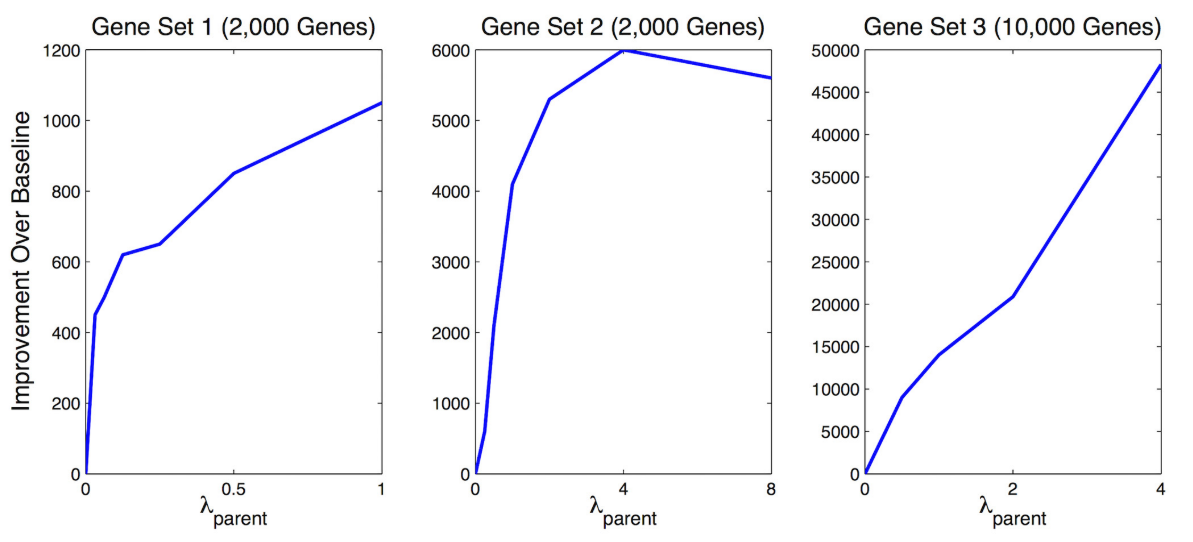
\includegraphics[width=0.85\linewidth]{slides/pierson_cv_likelihood.png}
  \caption{Improvement in cross-validated log likelihood over independent per-tissue graphical lasso ($\lambda_p=0$) as a function of the strength $\lambda_{\text{parent}}=\lambda_p$ of sharing along the tissue hierarchy, for three gene sets. Reproduced from \citet{pierson2015}.}
  \label{fig:pierson_cv}
\end{figure}

The tissue networks can then be compared, for example by finding clusters of genes that are densely connected in one tissue and not in others and testing each cluster for enrichment of gene sets with known function. \citet{pierson2015} report, for instance, a hippocampus-specific cluster enriched for synaptic vesicle genes. Such enrichments should be read with care. Enrichment tests need the right background set: genes expressed in brain are themselves enriched for synaptic functions, so a brain cluster tested against all genes will look enriched for synaptic terms whether or not the network is informative. More generally, validating an inferred network is hard because there is rarely a ground truth to compare against.

%======================================================================
\section{Network properties}
\label{sec:graph_properties}
%======================================================================

Once we have a network, whether measured or inferred, graph theory offers many summaries of its structure. Consider an undirected graph with $M$ nodes and adjacency matrix $\mA\in\{0,1\}^{M\times M}$, where $a_{ij}=a_{ji}=1$ if there is an edge between nodes $i$ and $j$ and $a_{ii}=0$. Let $|\mathcal{E}|=\sum_{i<j}a_{ij}$ be the number of edges. The \emph{degree} of node $i$ is the number of edges it has, $k_i=\sum_ja_{ij}$. Some properties describe the whole network and others describe individual nodes.

\begin{itemize}
  \item \emph{Density} (or sparsity). An undirected graph has $M(M-1)/2$ possible edges (a directed graph without self-loops has $M(M-1)$), and the density is $|\mathcal{E}|/\binom{M}{2}$. The number of possible edges grows as $O(M^2)$. A family of networks is called \emph{sparse} if the number of edges grows more slowly, for example as $O(M)$ or $O(M\log M)$, so that the mean degree $2|\mathcal{E}|/M$ stays small. Biological networks are sparse in this sense.
  \item \emph{Diameter}. The distance $d(a,b)$ between nodes $a$ and $b$ is the number of edges on a shortest path between them. The diameter is the largest distance between any two nodes, $\max_{a,b}d(a,b)$, computed within a connected component, since the distance between disconnected nodes is infinite. All distances from one node can be computed by breadth-first search in $O(M+|\mathcal{E}|)$ time, so the diameter takes $O(M(M+|\mathcal{E}|))$.
  \item \emph{Clustering coefficient}. For node $i$ with $k_i\ge2$ neighbours, the local clustering coefficient is the proportion of pairs of its neighbours that are themselves connected,
  \begin{equation}
    C_i = \frac{\sum_{j<l}a_{ij}a_{il}a_{jl}}{k_i(k_i-1)/2}.
  \end{equation}
  In social terms, it is the proportion of your friends who are friends with each other. The average of $C_i$ over nodes measures how clumped the network is.
  \item \emph{Betweenness centrality}. Let $\sigma_{st}$ be the number of shortest paths between nodes $s$ and $t$, and $\sigma_{st}(v)$ the number of those that pass through node $v$. The betweenness centrality of $v$ is
  \begin{equation}
    b(v) = \frac{1}{\binom{M-1}{2}}\sum_{s<t,\; s\neq v\neq t}\frac{\sigma_{st}(v)}{\sigma_{st}},
  \end{equation}
  the proportion of shortest paths through $v$, averaged over all pairs of other nodes. Nodes with high betweenness are bottlenecks or hubs of a transport network; in the British rail network, London would have very high betweenness, since many journeys pass through it. Brandes' algorithm computes $b(v)$ for all nodes in $O(M|\mathcal{E}|)$ time~\citep{brandes2001}.
  \item \emph{Degree distribution}. The histogram of degrees across nodes, $p(k)$, the fraction of nodes with degree $k$.
\end{itemize}

Figure~\ref{fig:betweenness} shows a random spatial network with $\btwNodes$ nodes and $\btwEdges$ edges, colored by betweenness. Its density is $\btwDensity$, its diameter $\btwDiameter$ and its average clustering coefficient $\btwClustering$; the clustering is high because nodes are connected when they are near each other, so neighbours of a node tend to be near each other too. The nodes with the highest betweenness, up to $\btwMaxBC$, are those that connect otherwise separate regions.

\begin{figure}[tbp]
  \centering
  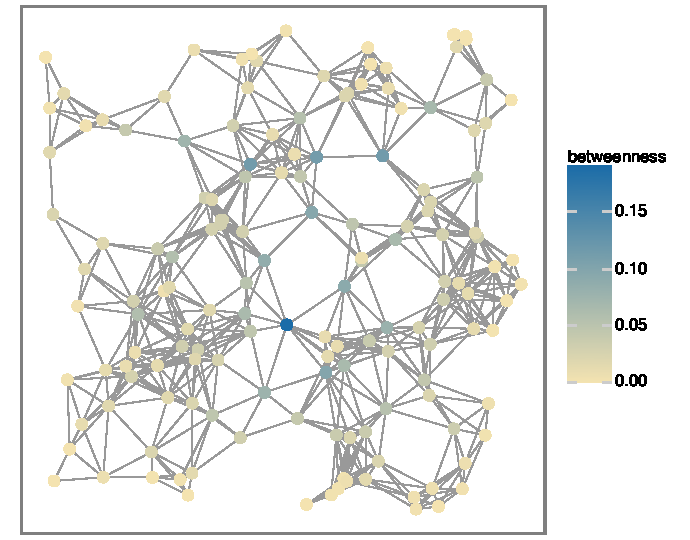
\includegraphics[width=0.6\linewidth]{betweenness.pdf}
  \caption{A random geometric graph (nodes placed uniformly in the unit square and connected if closer than 0.15; largest connected component shown), with nodes colored by betweenness centrality. Nodes that bridge different regions of the graph lie on many shortest paths.}
  \label{fig:betweenness}
\end{figure}

\subsection{Degree distributions and scale-free networks}

The simplest random graph model, the Erdős--Rényi model~\citep{erdos1959}, includes each of the $\binom M2$ possible edges independently with the same probability $p$. The degree of a node is then $\text{Binomial}(M-1,p)$, approximately Poisson with mean $(M-1)p$ for large $M$, and nodes with degree far above the mean are vanishingly rare. Many biological networks look different: most nodes have few edges, but a few hubs have very many. Such degree distributions are often described as \emph{scale-free}, following a power law
\begin{equation}
  p(k)\propto k^{-\gamma} \quad\Longleftrightarrow\quad \log p(k) = -\gamma\log k + \text{const},
\end{equation}
for some exponent $\gamma>0$, so that the distribution is a straight line on a log-log plot. \citet{reguly2006} found an approximately straight line for the degree distribution of literature-curated yeast genetic interactions, with the most connected genes having around 100 partners. A simple mechanism that produces power laws is \emph{preferential attachment}~\citep{barabasi1999}: the network grows one node at a time, and each new node connects to $m$ existing nodes chosen with probability proportional to their current degree, so that the rich get richer. Figure~\ref{fig:degree} compares the two models with the same number of nodes and the same mean degree. The largest degree is $\maxDegER$ under the Erdős--Rényi model and $\maxDegBA$ under preferential attachment.

\begin{figure}[tbp]
  \centering
  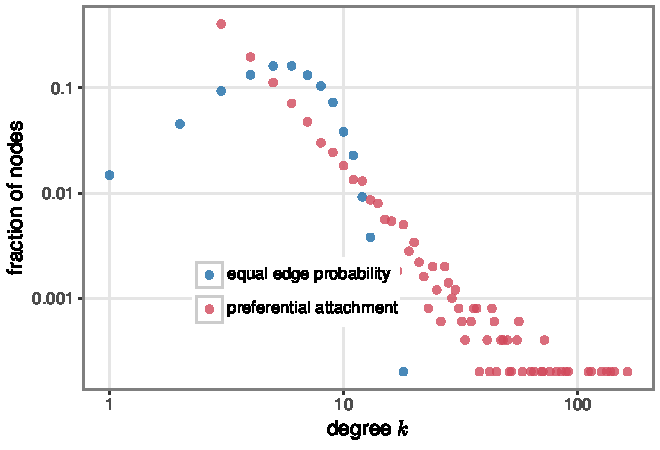
\includegraphics[width=0.6\linewidth]{degree_distribution.pdf}
  \caption{Degree distributions on log-log axes for two simulated networks with $M=5000$ nodes and mean degree 6: an Erdős--Rényi graph, in which every edge has equal probability (blue), and a preferential attachment graph (red, $m=3$). The Erdős--Rényi degree distribution is approximately Poisson and drops off quickly; preferential attachment gives an approximately straight line, a power law, with hubs of degree above 100.}
  \label{fig:degree}
\end{figure}

How widely biological networks are truly scale-free is debated. A systematic test of many networks found strong evidence for power laws in few of them~\citep{broido2019}, and degree distributions of measured networks are distorted by incomplete sampling: in PPI networks, well-studied proteins have more recorded interactions. It remains true that biological networks are much more heavy-tailed than the Erdős--Rényi model predicts.

%======================================================================
\section{Stochastic blockmodels}
\label{sec:sbm}
%======================================================================

The graphical lasso estimates a network from data. A different task is to model the structure of a given network, measured directly (like a PPI network) or estimated. A common structure is \emph{communities}: groups of nodes with many edges among themselves and fewer to the rest of the network. The \emph{stochastic blockmodel} (SBM)~\citep{holland1983,nowicki2001,abbe2018}, developed first for social networks, is a mixture model for this structure. It is to networks what a Gaussian mixture model, the probabilistic counterpart of $k$-means (Chapter 5), is to points.

\subsection{The generative model}

Let $K$ be the number of blocks (clusters, communities). The SBM generates an undirected network on $M$ nodes as follows.
\begin{enumerate}
  \item For each node $i=1,\dots,M$, draw a block assignment $c_i\sim\Cat(\vpi)$, where $\vpi\in\R^K$ is a probability vector; the simplest choice is $\vpi=[1/K,\dots,1/K]$, and $\vpi$ can instead be estimated or given a Dirichlet prior.
  \item For each pair of nodes $i<j$, draw the edge indicator
  \begin{equation}
    a_{ij}\mid c_i,c_j \sim \Bern\left(\eta_{c_ic_j}\right),
  \end{equation}
  and set $a_{ji}=a_{ij}$.
\end{enumerate}
Here $\veta\in[0,1]^{K\times K}$ is a symmetric matrix whose entry $\eta_{kl}$ is the probability of an edge between a node in block $k$ and a node in block $l$. A Bayesian version puts a prior $\eta_{kl}\sim\text{Beta}(a,b)$ on each entry. For example, with $K=3$,
\begin{equation}
  \veta = \begin{pmatrix} 0.5 & 0.01 & 0.01\\ 0.01 & 0.4 & 0.01\\ 0.01 & 0.01 & 0.6\end{pmatrix}
\end{equation}
describes three communities with dense connections within and sparse connections between them. A large diagonal is typical, an \emph{assortative} network, but nothing in the model requires it. A large off-diagonal entry describes two blocks that connect to each other more than to themselves, a \emph{disassortative} structure, as in a bipartite network between, say, enzymes and the metabolites they act on, or kinases and their substrates.

The joint probability of the assignments $\vc=(c_1,\dots,c_M)$ and the network is
\begin{equation}
  p(\mA,\vc\mid\vpi,\veta) = \prod_{i=1}^M\pi_{c_i}\prod_{i<j}\eta_{c_ic_j}^{a_{ij}}\left(1-\eta_{c_ic_j}\right)^{1-a_{ij}}.
  \label{eq:sbm_joint}
\end{equation}

\subsection{Inference}

As for a mixture model, the parameters can be fit by expectation maximization: an E step that infers the block assignments given $\veta$ and $\vpi$, and an M step that re-estimates $\veta$ and $\vpi$ given the assignments. There is one important difference from a Gaussian mixture. There, the posterior over assignments factorizes over data points. In the SBM each edge depends on the assignments of two nodes, so the posterior $p(\vc\mid\mA)$ couples all nodes and has $K^M$ configurations; the exact E step is intractable. The standard solution is \emph{variational EM}~\citep{daudin2008}: approximate the posterior by a factorized (mean-field) distribution $q(\vc)=\prod_iq_i(c_i)$, with $q_{ik}=q_i(c_i=k)$, and maximize the evidence lower bound
\begin{equation}
  \mathcal{L}(q,\vpi,\veta) = \E_q\left[\log p(\mA,\vc\mid\vpi,\veta)\right] - \E_q\left[\log q(\vc)\right].
\end{equation}
Taking the expectation of the log of~\eqref{eq:sbm_joint} under $q$,
\begin{equation}
  \E_q\left[\log p(\mA,\vc\mid\vpi,\veta)\right] = \sum_{i}\sum_kq_{ik}\log\pi_k + \sum_{i<j}\sum_{k,l}q_{ik}q_{jl}\left[a_{ij}\log\eta_{kl}+(1-a_{ij})\log(1-\eta_{kl})\right].
\end{equation}
\emph{M step.} Setting the derivative with respect to $\eta_{kl}$ to zero, and writing the sum over pairs as half a sum over ordered pairs $i\neq j$ to handle the symmetry of $\veta$,
\begin{equation}
  \hat\eta_{kl} = \frac{\sum_{i\neq j}q_{ik}q_{jl}a_{ij}}{\sum_{i\neq j}q_{ik}q_{jl}},
  \qquad \hat\pi_k = \frac1M\sum_iq_{ik},
\end{equation}
the expected number of edges between blocks $k$ and $l$ divided by the expected number of pairs. (The update for $\vpi$ uses a Lagrange multiplier for $\sum_k\pi_k=1$, as in Chapter 5.)

\emph{E step.} Holding all other factors fixed, the optimal $q_i$ is proportional to the exponentiated expected log joint, with the expectation taken over all other nodes,
\begin{equation}
  \log q_{ik} = \log\pi_k + \sum_{j\neq i}\sum_lq_{jl}\left[a_{ij}\log\eta_{kl}+(1-a_{ij})\log(1-\eta_{kl})\right] + \text{const},
\end{equation}
normalized so that $\sum_kq_{ik}=1$. Node $i$ is assigned to blocks whose connection pattern, given the soft assignments of all other nodes, best explains its row of $\mA$. These updates are iterated to convergence. Since $\mathcal{L}$ is not concave, several initializations, for example from spectral clustering (k-means on the leading eigenvectors of $\mA$), are used and the solution with the highest bound kept.

Figure~\ref{fig:sbm} applies this algorithm to a network of $M=120$ nodes simulated from an SBM with $K=4$ blocks: two assortative communities and a disassortative pair of blocks that connect mostly to each other. In the original node order, panel (a), no structure is visible. Ordering the nodes by their inferred block reveals it. The inferred blocks match the true ones exactly (adjusted Rand index $\sbmARI$), and, with blocks in the order shown in panel (b), the estimated edge probabilities are
\begin{equation}
  \hat\veta = \begin{pmatrix} \sbmEtaHat \end{pmatrix},
\end{equation}
close to the simulated values of 0.40 and 0.35 within the assortative blocks, 0.30 between the disassortative pair, and 0.03 to 0.04 elsewhere.

\begin{figure}[tbp]
  \centering
  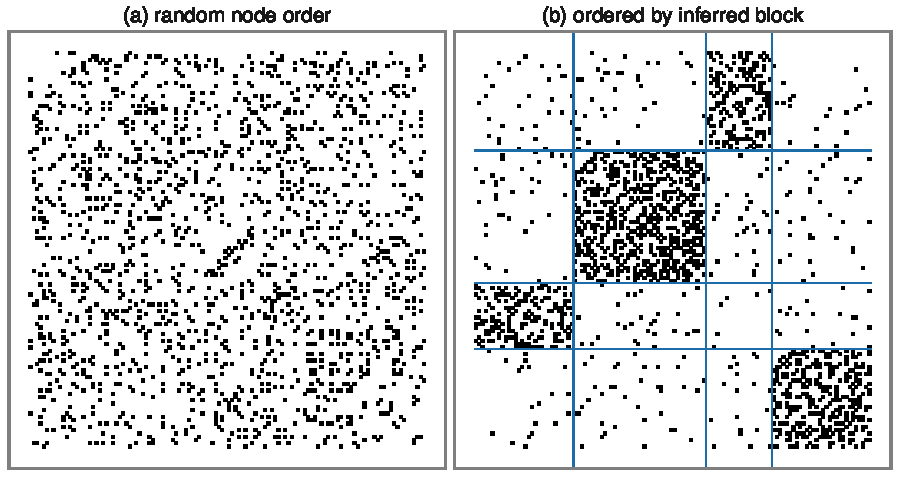
\includegraphics[width=0.85\linewidth]{sbm_adjacency.pdf}
  \caption{A stochastic blockmodel fit to a simulated network ($M=120$ nodes, $K=4$ blocks). Black entries of the adjacency matrix are edges. (a) Nodes in random order. (b) Nodes ordered by the blocks inferred by variational EM, with block boundaries in blue. Two blocks are assortative (dense diagonal blocks); the other two connect mainly to each other (dense off-diagonal blocks).}
  \label{fig:sbm}
\end{figure}

\subsection{Choosing the number of blocks}

The \emph{infinite relational model}~\citep{kemp2006} is a Bayesian nonparametric SBM. It places a Chinese restaurant process prior on the partition of nodes into blocks, which allows an unbounded number of blocks, and infers the number of blocks used by the data along with the assignments, typically by Markov chain Monte Carlo. It also handles several relations and directed relations at once. Bayesian nonparametric models of this kind have elegant mathematics but can be awkward in practice; a common alternative is to fit a model with generous $K$ and prune blocks that receive few nodes, or to compare values of $K$ by held-out likelihood or an information criterion.

\subsection{Predicting missing edges}

Because PPI networks have many false negatives, a natural use of a network model is \emph{link prediction}: scoring pairs of proteins with no recorded interaction by how likely an interaction is. Under a fitted SBM, the predicted probability of an edge between $i$ and $j$ is
\begin{equation}
  p(a_{ij}=1\mid\mA_{\text{obs}}) \approx \sum_{k,l}q_{ik}q_{jl}\hat\eta_{kl}.
\end{equation}
Blockmodels predict missing PPIs better than random guessing, though methods that use additional information, such as protein sequence, structure and co-expression, usually do better.

%======================================================================
\section{Mixed membership stochastic blockmodels}
\label{sec:mmsb}
%======================================================================

In the SBM, as in $k$-means, each node belongs to exactly one block. This is restrictive. In a social network you may have many friends at your university, but also friends from a sport you play and from a school you went to; no single community describes you. Many proteins likewise take part in several complexes or processes. Matrix factorization (Chapter 8) handles this by representing each object with several factors. \emph{Mixed membership} models instead represent each object by a probability distribution over clusters.

The mixed membership stochastic blockmodel (MMSB)~\citep{airoldi2008} replaces the block assignment $c_i$ of node $i$ with a membership vector $\vc_i\in\R^K$, with $c_{ik}\ge0$ and $\sum_kc_{ik}=1$. The generative model is as follows.
\begin{enumerate}
  \item For each node $i$, draw $\vc_i\sim\Dir([1,\dots,1])$. The Dirichlet distribution (Chapter 10) is the standard distribution on probability vectors; with all parameters equal to one it is uniform over the probability simplex.
  \item For each ordered pair of nodes $(i,j)$:
  \begin{enumerate}
    \item draw the block node $i$ acts in for this interaction, $z_{i\to j}\sim\Cat(\vc_i)$;
    \item draw the block node $j$ acts in, $z_{i\leftarrow j}\sim\Cat(\vc_j)$;
    \item draw the edge $a_{ij}\sim\Bern\big(\eta_{z_{i\to j},\,z_{i\leftarrow j}}\big)$.
  \end{enumerate}
\end{enumerate}
In the social example, my membership vector puts weight on ``Columbia faculty'' and on ``climbing''. For a particular person $j$, I draw one of my communities, say Columbia faculty; $j$, whose memberships are, say, Columbia faculty and cycling, draws one of theirs. The chance of a friendship is the entry of $\veta$ for that pair of communities, high if both drew the same community. Each pair gets its own draws, so different edges of a node can be explained by different communities.

Summing over the two indicators gives the probability of an edge given the memberships,
\begin{equation}
  p(a_{ij}=1\mid\vc_i,\vc_j,\veta) = \sum_{k=1}^K\sum_{l=1}^Kp(z_{i\to j}=k)\,p(z_{i\leftarrow j}=l)\,\eta_{kl} = \sum_{k,l}c_{ik}\eta_{kl}c_{jl} = \vc_i^\top\veta\,\vc_j .
\end{equation}
Collecting the memberships as rows of a matrix $\mathbf{C}\in\R^{M\times K}$, the matrix of edge probabilities is $\mathbf{C}\veta\mathbf{C}^\top$, a low-rank, non-negative factorization of the kind seen in Chapter 8. If every $\vc_i$ is a one-hot vector the MMSB reduces to the SBM.

Inference is again by variational EM, with an E step for the indicators $z$ (and the posterior over the memberships $\vc_i$) and an M step for $\veta$. \citet{airoldi2008} applied the MMSB to a yeast PPI network and used the inferred memberships to predict proteins' functional annotations, more accurately than random annotation baselines. The MMSB has the same structure as latent Dirichlet allocation (LDA)~\citep{blei2003}, the standard topic model for text before large language models: a document has a distribution over topics and each word is generated from one topic drawn from it, as a node has a distribution over communities and each interaction uses one community drawn from it. Figure~\ref{fig:sbm_gm} compares the SBM and MMSB as graphical models.

\begin{figure}[tbp]
  \centering
  \begin{tikzpicture}[>=Stealth, every node/.style={font=\small},
      lat/.style={draw, circle, minimum size=0.85cm, inner sep=1pt},
      obs/.style={draw, circle, fill=gray!25, minimum size=0.85cm, inner sep=1pt},
      par/.style={draw, rectangle, minimum size=0.6cm, inner sep=2pt}]
    \node at (-0.5,3.0) {(a) SBM};
    \node[par] (pi) at (1.5,2.3) {$\vpi$};
    \node[lat] (ci) at (0.5,1.0) {$c_i$};
    \node[lat] (cj) at (2.5,1.0) {$c_j$};
    \node[obs] (a) at (1.5,-0.4) {$a_{ij}$};
    \node[par] (eta) at (3.4,-0.4) {$\veta$};
    \draw[->] (pi) -- (ci); \draw[->] (pi) -- (cj);
    \draw[->] (ci) -- (a); \draw[->] (cj) -- (a); \draw[->] (eta) -- (a);
    \begin{scope}[xshift=6.3cm]
      \node at (-1.1,3.0) {(b) MMSB};
      \node[lat] (ci) at (0.3,2.3) {$\vc_i$};
      \node[lat] (cj) at (2.9,2.3) {$\vc_j$};
      \node[lat] (zi) at (0.3,0.95) {$z_{i\to j}$};
      \node[lat] (zj) at (2.9,0.95) {$z_{i\leftarrow j}$};
      \node[obs] (a) at (1.6,-0.4) {$a_{ij}$};
      \node[par] (eta) at (3.6,-0.4) {$\veta$};
      \draw[->] (ci) -- (zi); \draw[->] (cj) -- (zj);
      \draw[->] (zi) -- (a); \draw[->] (zj) -- (a); \draw[->] (eta) -- (a);
    \end{scope}
  \end{tikzpicture}
  \caption{Graphical models for one pair of nodes $(i,j)$. Shaded circles are observed, open circles latent, squares parameters. (a) In the stochastic blockmodel each node has a single block $c_i$, shared by all its edges. (b) In the mixed membership SBM each node has a membership vector $\vc_i$, and each interaction draws its own blocks $z_{i\to j}$ and $z_{i\leftarrow j}$ from the two nodes' memberships.}
  \label{fig:sbm_gm}
\end{figure}

%======================================================================
\section{Summary}
%======================================================================

\begin{itemize}
  \item ``Network'' means different things in biology; always ask what the nodes and edges are. Gene regulatory networks link transcription factors to their target genes (directed, signed); co-expression networks link co-regulated genes (undirected, inferred); protein-protein interaction networks link physically binding proteins; genetic interaction networks link genes whose double mutants deviate from the multiplicative expectation $f_if_j$; metabolic networks link metabolites through enzymatic reactions; signaling networks link kinases and other signaling molecules.
  \item Correlation mixes direct and indirect association. The partial correlation of two variables given all others is $-\theta_{ij}/\sqrt{\theta_{ii}\theta_{jj}}$, where $\mTheta$ is the precision matrix; for Gaussian data a zero entry means conditional independence.
  \item The graphical lasso estimates a sparse precision matrix by minimizing $-\log|\mTheta|+\tr(\mTheta\hSigma)+\lambda\|\mTheta\|_1$. It is convex, works when $N<P$, is fit by block coordinate descent over lasso subproblems, and $\lambda$ can be chosen by cross-validated likelihood.
  \item Networks for related tissues can be estimated jointly by penalizing differences between precision matrices along a tissue hierarchy, which improves held-out likelihood in GTEx.
  \item Network properties from graph theory include density, diameter, clustering coefficient, betweenness centrality and the degree distribution, which in biological networks is heavy-tailed.
  \item Stochastic blockmodels are mixture models for networks, fit by variational EM, and can predict missing edges. Mixed membership SBMs let each node belong to several communities, with edge probability $\vc_i^\top\veta\vc_j$.
\end{itemize}

%======================================================================
\section*{Exercises}
%======================================================================

\begin{enumerate}
  \item Let $x_1\sim\Normal(0,1)$, $x_2=ux_1+\epsilon_2$ and $x_3=vx_2+\epsilon_3$ for scalars $u,v\neq0$, with independent $\epsilon_2,\epsilon_3\sim\Normal(0,1)$. Compute the covariance matrix $\mSigma$ and the precision matrix $\mTheta$ of $(x_1,x_2,x_3)$. Show that $\Sigma_{13}\neq0$ but $\theta_{13}=0$, and interpret.
  \item Using the block matrix inversion formula, show that the coefficients of the population regression of $x_A$ on all other variables are $\beta_{Aj}=-\theta_{Aj}/\theta_{AA}$ and that the residual variance is $1/\theta_{AA}$.
  \item Show that $-\log|\mTheta|$ is convex on the set of positive definite matrices. (Hint: restrict to a line $\mTheta+t\mathbf{V}$ and write the function in terms of the eigenvalues of $\mTheta^{-1/2}\mathbf{V}\mTheta^{-1/2}$.)
  \item For the tissue hierarchy objective~\eqref{eq:gtex_objective} with $K=2$ tissues joined at a root, show that for fixed leaves the optimal root matrix is $\frac12(\mTheta^{(1)}+\mTheta^{(2)})$, and that the penalty then equals $\frac{\lambda_p}{2}\|\mTheta^{(1)}-\mTheta^{(2)}\|_2^2$.
  \item Compute the degree, clustering coefficient and betweenness centrality of every node in a star graph (one centre connected to $M-1$ leaves) and in a cycle of $M$ nodes. What are the diameters?
  \item Derive the M-step update for $\eta_{kl}$ in the SBM and show that when the $q_{ik}$ are one-hot it is the number of edges between blocks $k$ and $l$ divided by the number of node pairs between them.
  \item Implement the graphical lasso with cross-validation on the expression of a few hundred genes from one GTEx tissue. How does the number of edges at the cross-validated $\lambda$ change if you first regress out the top five principal components?
\end{enumerate}

\bibliographystyle{abbrvnat}
\bibliography{chapter09}
\end{document}
